\documentclass[a4paper,10pt,twocolumn]{paper}
%\documentclass[a4paper,11pt,onecolumn]{article}

\usepackage{natbib}
\usepackage{rotating}
\usepackage[font={small}]{caption}
\usepackage{array}
\usepackage{booktabs}
\usepackage{authblk}
\usepackage{color}
\usepackage{xcolor}
\usepackage{lineno}
\usepackage{url}
\usepackage[margin={2cm,2cm}]{geometry}

\title{The seismic signature of upper-mantle plumes: application to the northern East-African Rift}

\author[1]{Chiara Civiero}
\author[2]{John J.~Armitage}
\author[3]{Saskia Goes}
\author[4]{James O.~S.~Hammond}
%\author{[ngu]{Lo{\"i}c Fourel}}

%\cortext[cor1]{Corresponding author, email@address}

\affil[1]{Dublin Institute for Advanced Studies (DIAS), Dublin D02 Y006, Ireland}
\affil[2]{Dynamique des Fluides G{\'e}ologiques, Institute de Physique du Globe de Paris, Paris, France}
\affil[3]{Department of Earth Science and Engineering, Imperial College London, London, UK}
\affil[4]{Department of Earth and Planetary Sciences, Birkbeck, University of London, London, UK}
%\address[ngu]{Norway}

\begin{document}

\maketitle
\bibliographystyle{elsart-harv}

\begin{abstract}
Several recent seismic and numerical studies proposed that below some hotspots secondary smaller-scale upper-mantle plumelets rise from a regional thermal boundary layer below 660\,km depth, fed by a deeper plume source. We recently found tomographic evidence of several small upper-mantle upwellings, spaced by several 100 km, rising through the transition zone below the northern East-African Rift. To better test this interpretation, we run 3D numerical simulations of mantle convection for Newtonian and non-Newtonian rheologies within a Cartesian box, for both thermal instabilities rising from the lower boundary, and the destabilisation of a thermal anomaly initially placed at the base of the box. The thermal structures are converted to seismic velocities using a mineral-physics approach. Synthetic resolution tests are then conducted for the same P- and S- data distribution and inversion parameters as our original teleseismic travel-time tomography. The models predict simultaneous plumelets in different stages of their evolution rising from a hot boundary layer located in the topmost lower mantle, resulting in seismic structure that looks substantially more complex than the simple vertical cylinders that are often anticipated. From the selection of models we find that the destabilisation of a $100\,^{\circ}$C, 100 km thick thermal anomaly with a non-Newtonian rheology, most closely matches the spatial and temporal distribution of seismic anomalies below the rift system. However, the destabilisation of a $200\,^{\circ}$C anomaly best matches the magnitudes of the anomalies. Finally, we find that for reasonable upper-mantle viscosities, the synthetic plume tomography is similar in scale, variability of anomaly shape, and vertical correlation variation to the actual P- and S-wave tomography of the northern East-African Rift, providing further support for the existence of upper-mantle plumelets below the region.
\end{abstract}

\section{Introduction}

Volcanic rifting is undoubtedly related to the thermal state of the mantle during extension and decompression melting \citep[e.g.][]{white-1989}, and the thermal state of the mantle can be estimated from seismic wave speeds derived from inverse models. The East African Rift is the largest active volcanic rift zone on the planet. However despite the clear evidence for decompression melting, there have been conflicting interpretations of the thermal state of the mantle below Afar and the Main Ethiopian Rift. The low seismic velocity inverted from surface waves is consistent with a hotter than average mantle, $1450\,^{\circ}$C, or roughly $100\,^{\circ}$C hotter than normal mantle \citep{armitage-etal-epsl-2015}. However, a S-wave tomographic model of the Afar region found that at around 400\,km depth, the S-wave velocity was lower than could be explained by a simple $100\,^{\circ}$C thermal anomaly \citep{thompson-etal-2015}. This can be explained if there is a certain degree of very deep partial melting which becomes retained within the mantle \citep{thompson-etal-2015}.

Interpretations of inverse seismic models, such as the presence of very deep melt, or a vertically rising thermal plume, are rarely tested. The seismic velocity structure below the East African Rift (EAR) derived from tomographic models is complex \citep{civiero-etal-2015,civiero-etal-2016}. In fact, the EAR is not unique in terms of complexity: Several recent tomographic studies have found evidence of plume complexity, including possible branching \citep{rickers-etal-2013}, and  triggering of secondary upper-mantle plumes above a lower-mantle source \citep{civiero-etal-2018,goes-etal-1999,saki-etal-2015}. The apparent complexity from tomographic inversions has been interpreted to represent secondary instabilities, such as small plumes, or plumelets, rising from a stalled larger thermal anomaly is appealing given that secondary plumes have been shown to occur within laboratory experiments \citep[e.g.]{kumagai-etal-2007}, however the hypothesis that follows from the interpretation of seismic tomographic models needs to be tested. In this study we will explore if small-scale plumes, or \emph{plumelets}, are consistent with seismic observations. We develop a workflow to model physically plausible plumelet scenarios based on regional mantle flow. These physical structures are converted to seismic structures and are the re-resolved at the scale of the seismic experiment. This allows us to test the hypothesis that the apparent complexity in seismic tomographic images is due to complex plume-like structures within the upper mantle.

Only a few previous studies have tested the tomographic results against dynamic models to understand the nature and origin of mantle plumes, with very few using full resolution tests. \cite{boschi-etal-2007} and \cite{styles-etal-2011} did a comparison of global and regional plume models against global tomography to get an overview of how many plumes might exist. \cite{davaille-etal-2005} looked over a large region encompassing all of African and surrounding hotspots below the Atlantic and Indian Ocean, and qualitatively compared plume styles predicted from analogue models. Structures from dynamic plume models have been used by \cite{hwang-etal-2011} and \cite{maguire-etal-2016} to illustrate how wavefront healing may mask the travel-time signatures of plumes below 1000 km depth. MAGUIRE ET AL., (2018) To better understand plume resolution given the limitations of network design... \cite{ballmer-etal-2013} performed a regional study focusing on Hawaii and found that numerical models of a complex thermo-chemical plume are compatible with the tomographic images of the upper mantle below the islands.

In this paper, we numerically generate upper-mantle upwellings from both a steady-state thermal boundary layer and from a local hot layer below 660\,km depth using Earth-like parameters. We will first analyse plume scales and strength in the numerical models as a function of Rayleigh number and temperature contrast across the hot thermal boundary layer. Next, we convert the thermal models to seismic velocity using thermo-dynamic methods that account for the effects of temperature, pressure, phase, composition and anelasticity \citep{cobden-etal-2008,goes-etal-2004,styles-etal-2011b}. We then use these seismic structures as input for synthetic resolution tests using the same data distribution and inversion scheme and parameters as in \cite{civiero-etal-2015,civiero-etal-2016}. Finally, we compare the simulated convective instabilities with our seismic observations to find (a) the parameters of the models needed to justify the spacing, scale and amplitude the seismic anomalies imaged below the rift system; (b) the type and location of the thermal boundary layer able to generate such instabilities in the upper mantle; (c) the most plausible geometry and thus the stage in temporal evolution of the two mantle plumes below Afar and MER.

\subsection{Tomography on the northern East-African Rift}

\begin{figure*}
\centering
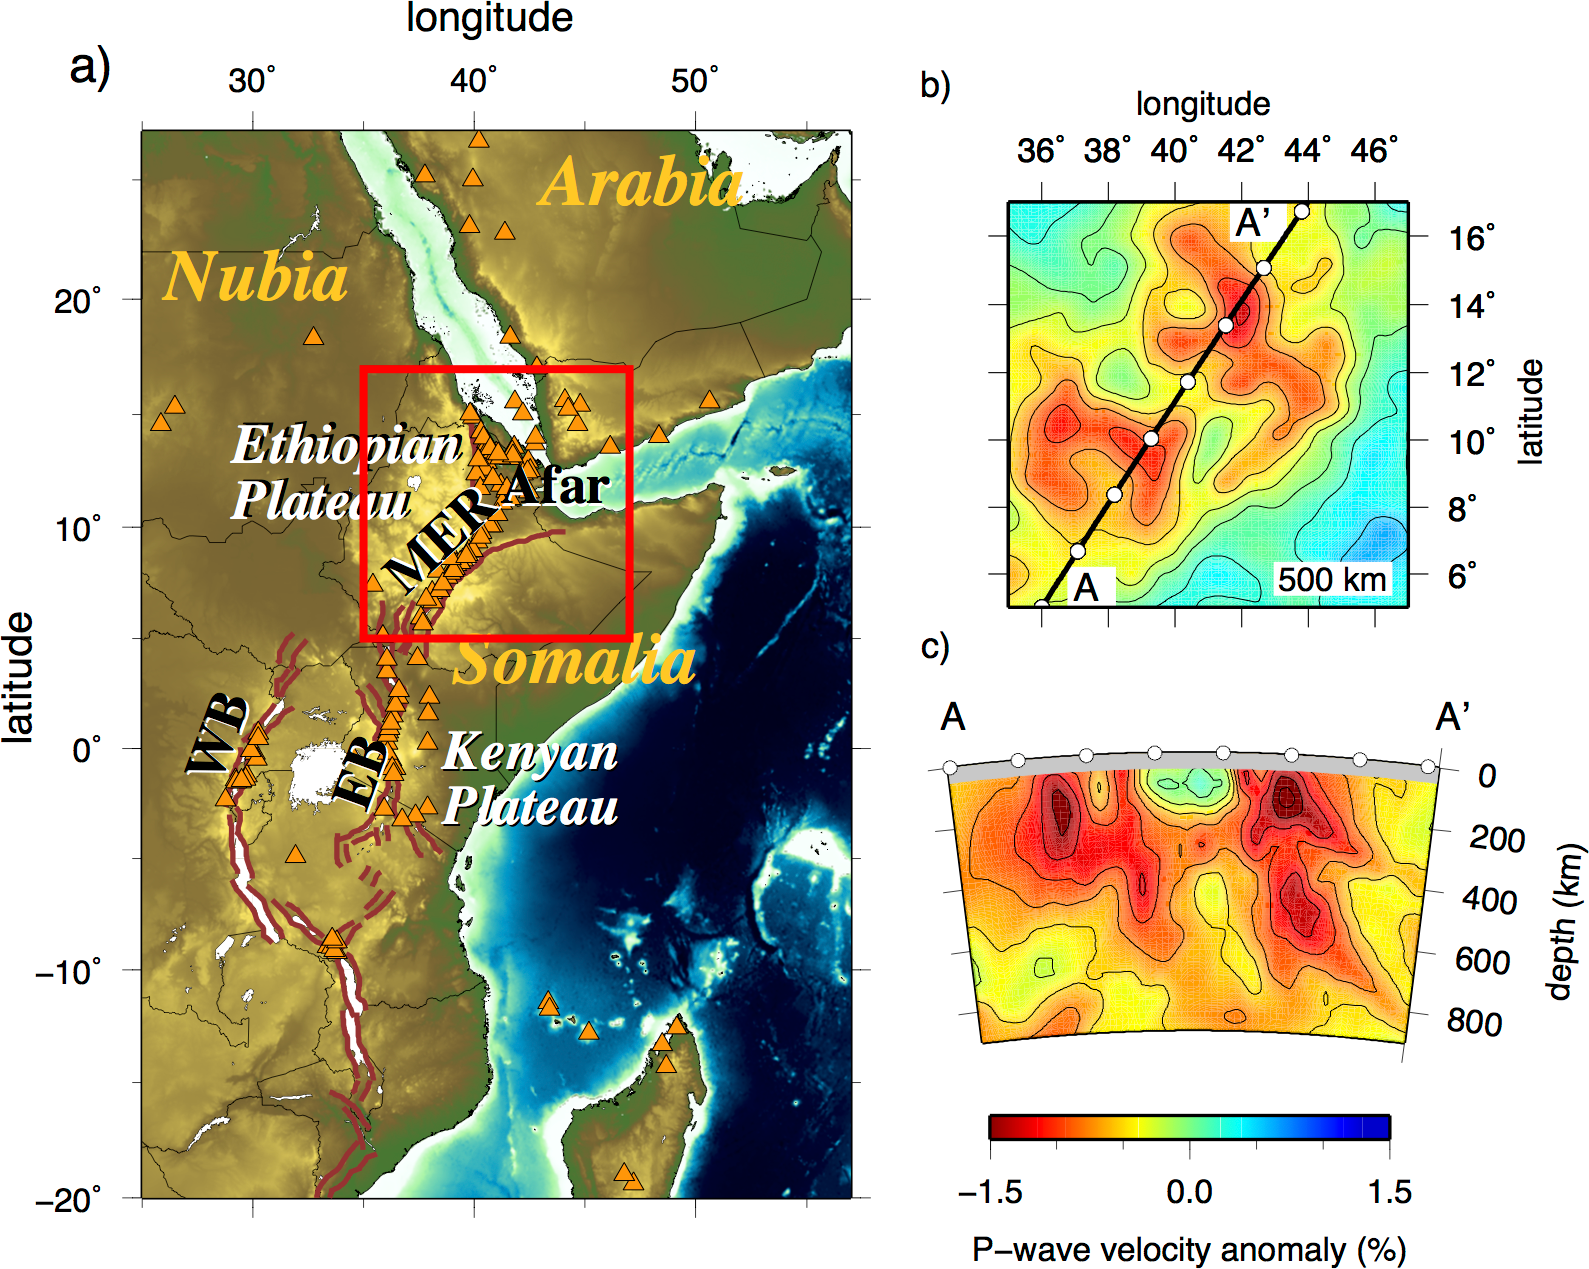
\includegraphics[width=11cm]{../figures-working/fig01.png}
\caption{Study area and tomography: (a) East African rift tomographic model, Holocene volcanoes, and active fault zones. Stations used were distributed all across the area shown (see supplement for station locations), but good resolution was obtained in the study area in the black box. (b) horizontal depth slice through the undamped P model, NEAR-P15 at 500 km depth. The black line indicates the orientation of the cross-section in c. (c) vertical cross-section through the undamped P model NEAR-P15. The cross-section illustrates two clusters of low velocity anomalies below Afar and west of the MER extending to the base of the transition zone.}
\label{fg:1}
\end{figure*}

The P- and S-wave tomography performed by \cite{civiero-etal-2015,civiero-etal-2016} imaged the mantle structure below the northern EAR using seismic stations deployed along the rift from Saudi Arabia in the north to Madagascar in the south (Fig.~\ref{fg:1}). The study region comprises Afar and the Main Ethiopian rift (MER), i.e., the northern end of EAR. This area is characterised by a topographic swell (the Ethiopian Plateau), 30\,Myr old flood basalts, and currently active volcanism and extensional faulting (Fig. 1a). Seismic stations that were used are from 26 different temporary and permanent arrays that span the region from Saudi Arabia to Madagascar. This wide aperture allows for high resolution from 50\,km below the study area in the box in Fig.~\ref{fg:1}a, from $\sim50$\,km down to between 700 and 800\,km depth.

\cite{civiero-etal-2015,civiero-etal-2016} performed teleseismic travel-time tomography using the method of \cite{vandecar-etal-1995}, on a data set of 16420 relative P travel times and 16569 relative S and SKS travel times. The preferred tomographic results include moderate damping to a regional surface-wave model (Fishwick, 2010) down to 300 km depth, where the limited number of crossing teleseismic rays does not provide good vertical resolution. These models, NEAR-P15 (for P-waves) and NEAR-S16 (for S- and SKS-waves), were obtained with regularisation parameters that provide a balance between misfit reduction and not overfitting the data beyond the data error estimates (using flattening=4800, smoothing= 153,600).

As illustrated in Fig.~\ref{fg:1}b and c, the tomographic inversion recovered two clusters of low-velocity anomalies, below Afar and MER, that extend from about 200 km depth to the topmost lower mantle. The P-wave model clear illustrates that the two clusters are separate features, and required to extend through the transition zone. The sub-lithospheric low-velocities have been attributed to the spreading of plume material below the lithosphere, with local contributions from melt \citep{civiero-etal-2015,civiero-etal-2016}. The deeper structures (300-660\,km depth) were interpreted as plume tails. Below 700\,km depth, the structure changes, in particular in the P-wave model where resolution extends somewhat deeper than in the S-wave model.

\subsection{Constraints on plume spacing}

Various studies have suggested that hotspot or volcanic clusters may share the same root zone. \cite{kumagai-etal-2007} proposed that the French Polynesian hotspots (Tahiti-Macdonald-Pitcairn), the Canaries-Cape Verde-Azores-Great Meteor hotspots and the Marion-Crozet hotspots share a source comprising ponded material below 660\,km depth seismic discontinuity. \cite{saki-etal-2015}, based on the analysis of transition-zone discontinuity topography from PP and SS precursors, also proposed that the Canaries-Cape Verde and Azores share a source layer below the transition zone. Tomographic images by \cite{rickers-etal-2013} indicate that Iceland and Jan Mayen are two branches of a common plume below 1300\,km. In all these cases, the spacing between hotspots is around 1000-150\,km. \cite{chang-2011} imaged possible plume conduits below Afar, Kenya and northern Saudi Arabia that are separate down to at least 1500\,km depth. Again spacing between these proposed plumes is about 1500\,km.

Other examples suggest a plume spacing of hundreds of kilometers: These include our inferred Afar and MER plumelets which are separated by 400-600\,km \citep{civiero-etal-2015,civiero-etal-2016}, proposed \emph{baby plumes} below the European hotspots (Eifel, Massif Central, Bohemian Massif, upper Rhine Graben, Brest Graben; \citealp{goes-etal-1999,granet-etal-1995}, which are spaced 250-400\,km. Furthermore, spacing between active volcanoes within the Canaries, Cape Verde, Society Islands is between 50 and 300\,km.

\subsection{Dynamic controls on plume spacing}

The spacing of thermal plumes that form naturally in laboratory experiments of Rayleigh B{\'e}nard convection, where the strongly temperature dependent viscous fluid is heated from the base and cooled from the top is a function of the aspect ratio of the rectangular tank and the local Rayleigh number \citep{androvandi-etal-2011}. For fluids that have a viscosity that is an exponential function of temperature, the wavelength, or plume spacing, is observed to decrease with $Ra$ as $\lambda/H \propto Ra^{1/3}$, where $H$ is the height of the experimental tank \citep{androvandi-etal-2011}. In numerical experiments where the fluid is assumed to be isoviscous, the reduction in wavelength takes the form $\lambda/H \propto Ra^{1/6}$ \citep{zhong-2005,galsa-2007}. If we assume that the plumes initiate at $\sim 1000$\,km depth, then the spacing of the plumes would be of the order of 1000 km or less, for a local $Ra > 10^{5}$ \citep{androvandi-etal-2011}. Therefore, it follows that if the stagnation of large whole mantle plumes at shallow depth leads to the formation of secondary plumes (plumelets) due to the increased temperature at the boundary \citep[e.g.][]{kumagai-etal-2007}, then the spacing will be a function of the depth at which the stagnation occurs.

For the destabilisation of a layer of hot material, or the development of Rayleigh Taylor instabilities, the growth of the instability should be largest for the characteristic wavelength defined by the aspect ratio of the domain. From linear scaling analysis of the destabilisation of a layer equal to one tenth of the height of the region, $H$, the characteristic wavelength is $\lambda = 0.37H$ \citep{schmeling-1987}. This calculation is for two materials of the same viscosity. It was subsequently demonstrated that in 2D systems the final dominant wavelength is not necessarily equal to the characteristic wavelength if there was an initial perturbation to the system \citep{schmeling-1987}. That aside, if we assume a thin layer 100\,km thick of hot mantle material ponds at the 660\,km depth seismic discontinuity, then the characteristic wavelength of the plumelets would be on the order of 200\,km. Given the impact of the initial configuration on the estimate of plume wavelength, we will numerically model both Rayleigh B{\'e}nard and Rayleigh Taylor instabilities for Newtonian and non-Newtonian rheologies.

\section{Dynamic models methods}

\subsection{Numerical models set-up}

We solve Stokes equations using the numerical model Stag3D \citep{tackley-1998} for the flow of a highly viscous fluid within a Cartesian domain of aspect ratios 3x3x1, 4x4x1, and 6x6x1, and the model is 700\,km deep. Mechanical boundary conditions are free slip on all sides and of fixed temperature at the top and bottom. Temperature boundaries on the sides are of zero gradient. Tracers are used to make material at the top - between 0 and 0.14H depth - buoyant, by assigning them a buoyancy number, $B$, which equals the thermal over chemical density anomaly: $B = \Delta\rho_{c}/\Delta\rho_{T} = 0.5$ \citep{fourel-2009}. This depth range will comprise most of the upper thermal boundary layer that forms as the model evolves. This minimizes lithospheric participation in the convection pattern and allows us to focus on plume scales and geometry.

Temperature in the asthenosphere is initially set to $1350\,^{\circ}$C, the assumed background mantle potential temperature. At between 0 and 100\,km depth, temperature increases linearly from $0\,^{\circ}$C  to $1350\,^{\circ}$C. At the bottom of the model we explore two setups:
\begin{itemize}
\item A hot lower boundary condition of $1350{\rm^{\circ} C} + \Delta T_{e}$, where $\Delta T_{e}$ is the excess temperature.
\item A basal hot layer, 100\,km thick thick, of temperature $\Delta T_{e}$ is included in the initial condition, and the lower boundary temperature is held at $1350\,^{\circ}$C.
\end{itemize}
The former lower boundary condition will lead to Rayleigh B{\'e}nard convection, while the latter initial condition will destabalise in the form of Rayleigh Taylor instabilities.

The form of the convective instabilities will be determined by the rheology of the upper mantle. We test two different dominant mechanisms for mantle creep, diffusion and dislocation creep, which can be expressed as a Newtonian and a non-Newtonian rheology. The first rheology we take is an idealised temperature dependent Newtonian material written as,
\begin{equation}
\eta = \eta_{0}A_{ref}exp\left(\frac{E}{RT}\right)
\end{equation}
where $\eta_{0}$ is the scaling viscosity, $A_{ref} = 2.2\times10-5$ is the pre-factor, $E = 120\rm\,kJ\,mol^{-1}$ is the activation energy, $R=8.31$ is the ideal gas constant and $T$ is mantle potential temperature. The activation energy, which was determined empirically for the upper mantle to achieve agreement between calculations and observations of lithosphere plate flexure, is a factor of 3 lower than experimentally derived estimates \citep{korenaga-jgr-2008,watts-2000}. However, as shown by \cite{christensen-1984} and \cite{jaupart-2011}, a small value for the activation energy may be regarded as a convenient way to approximate nonlinear diffusion creep with a Newtonian analogue.

The second rheology we consider is a strain weakening non-Newtonian temperature and pressure-dependent creep law,
\begin{equation}
\eta = \eta_{0}A_{ref}^{\frac{1}{n}}exp\left(\frac{E+pV}{nRT}\right) \dot{I_{2}}^{\frac{1-n}{n}}
\end{equation}
where the pre-factor $A_{ref} = 1.47\times10^{-16}$ for a reference strain rate of $10^{-15}\rm\,s^{-1}$, $E = 523\rm\,kJ\,mol^{-1}$, activation volume $V = 4\rm\,cm^{3}\,mol^{-1}$, stress exponent $n=3.6$ \citep{korenaga-jgr-2008}, and $\dot{I_{2}}$ is the second invariant of the deviatoric strain rate tensor. Finally in both models the scaling viscosity, $\eta_{0}$, is set by the initial Rayleigh number,
\begin{equation}
Ra = \frac{\alpha g\rho_{m}\Delta TH^{3}}{\kappa \eta_{0}}
\end{equation}
where $H$ is the height of the model domain and $\Delta T$ is the temperature difference across the model domain from top to the bottom. The remaining constants are listed in Table \ref{tb:1}. We explore initial $Ra$ of $10^6$ to $10^8$. The various models are listed in Table \ref{tb:2}.

\begin{table*}
\centering
\caption{Model parameters}
\label{tb:1}
\begin{tabular}{c c c}
\hline
Parameter & Value & Description \\
\hline
$B$       & 0.5   & Bouyancy number for the lithosphere \\
$g$       & $9.8\rm\,m\,s^{-2}$ & Acceleration due to gravity \\
$H$       & 700\,km & Model depth \\
$p$       &       & Pressure \\
$Ra$      &       & Initial Rayleigh number \\
$T$       &       & Temperature \\
$\Delta T$& $1350\,^{\circ}$C & Asthenosphere temperature \\
$\Delta T_{e}$&   & Temperature anomaly \\
$\alpha$  & $3.3\times10^{-5}\rm\,K^{-1}$ & Coefficient of thermal expansion \\
$\kappa$  & $10^{-6}\rm\,m^{2}\,s^{-1}$ & Thermal diffusivity \\
$\rho_{m}$& $3340\rm\,kg\,m^{3}$ & Mantle density \\
$\eta_{0}$&       & Scaling viscosity \\
\hline
\multicolumn{3}{c}{Newtonian Rheology} \\
\hline
$E$       & $120\rm\,kJ\,mol^{-1}$ & Activation energy \\
$A_{ref}$ & $2.2\times10-5$ & Normalizing factor \\
\hline
\multicolumn{3}{c}{Non-Newtonian Rheology} \\
\hline
$E$       & $523\rm\,kJ\,mol^{-1}$ & Activation energy \\
$V$       & $4\rm\,cm^{3}\,mol^{-1}$ & Activation volume \\
$n$       & 3.6 & Stress exponent \\
$A_{ref}$ & $1.47\times10^{-16}$ & Normalizing factor \\
\hline
\end{tabular}
\end{table*}

\begin{table*}
\centering
\caption{List of models}
\label{tb:2}
\begin{tabular}{c c c c c c c}
\hline
Name & Type & Ra & $\Delta T_{e}$  & Newtonian & Non-Newtonian & Aspect ratio \\
     &      &    & ($^{\circ}$ C)        &           &               & (resolution) \\
\hline
N1   & Rayleigh & $6\times10^5$ & 100 & x & & 6x6x1 \\
     & B{\'e}nard   &               &     &            & & (384x384x64) \\
N2   & Rayleigh & $2\times10^6$ & 100 & x & & 6x6x1 \\
     & B{\'e}nard   &               &     &            & & (384x384x64) \\
N3   & Rayleigh & $6\times10^6$ & 100 & x & & 6x6x1 \\
     & B{\'e}nard   &               &     &            & & (384x384x64) \\
N4   & Rayleigh & $6\times10^7$ & 100 & x & & 6x6x1 \\
     & B{\'e}nard   &               &     &            & & (384x384x64) \\
N5   & Rayleigh & $6\times10^5$ & 100 & & x & 6x6x1 \\
     & B{\'e}nard   &               &     &            & & (384x384x64) \\
N6   & Rayleigh & $6\times10^6$ & 100 & & x & 6x6x1 \\
     & B{\'e}nard   &               &     &            & & (384x384x64) \\
N7   & Rayleigh & $6\times10^6$ & 100 & & x & 3x3x1 \\
     & Taylor   &               &     &            & & (192x192x64) \\
N8   & Rayleigh & $6\times10^6$ & 100 & & x & 4x4x1 \\
     & Taylor   &               &     &            & & (512x512x128) \\
N9   & Rayleigh & $6\times10^6$ & 200 & & x & 4x4x1 \\
     & Taylor   &               &     &            & & (512x512x128) \\
N10  & Rayleigh & $6\times10^6$ & 400 & & x & 4x4x1 \\
     & Taylor   &               &     &            & & (512x512x128) \\   
\hline
\end{tabular}
\end{table*}

\section{Dynamic models – plume scales and styles}

\begin{figure*}
\centering
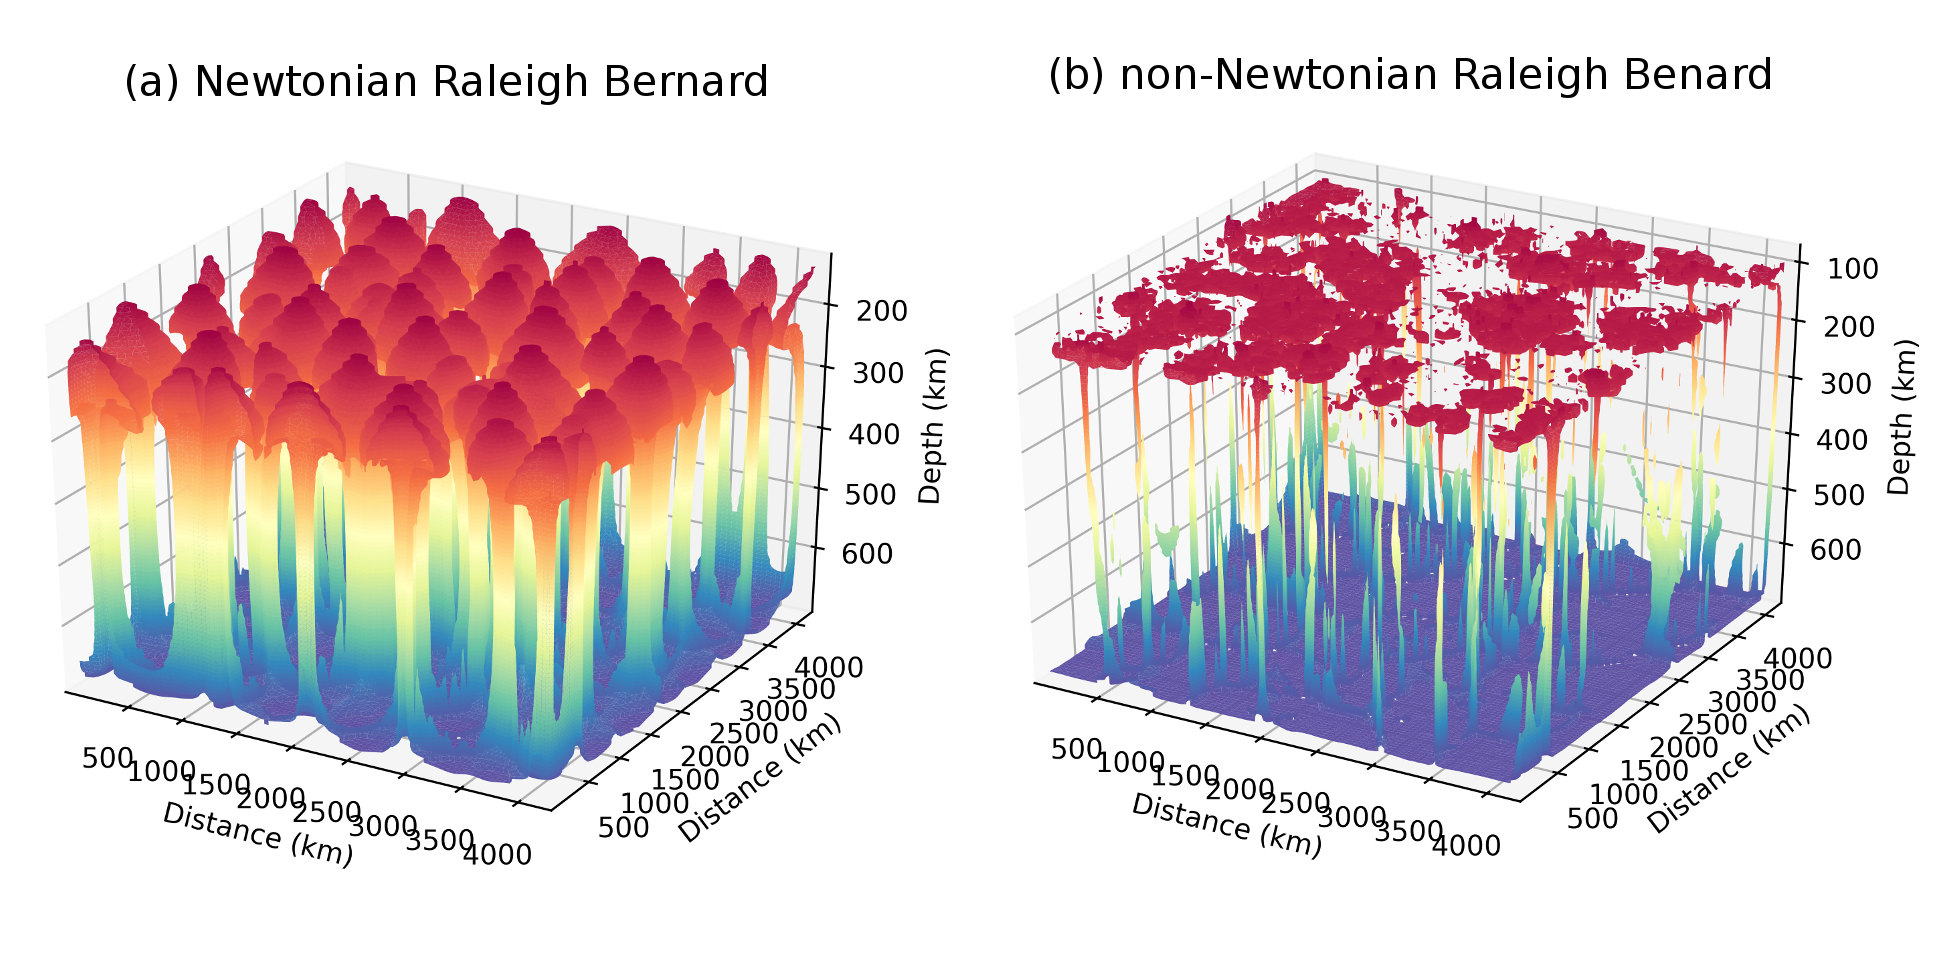
\includegraphics[width=16cm]{../figures-working/comparison.png}
\caption{Surface plots of the 1\,\% thermal anomaly (corresponding to a temperature of $1363.5\,^{\circ}$C) coloured by depth. In both models the $Ra = 6\times10^{6}$, models N3 and N6 in Table \ref{tb:2}. (a) Raleigh B{\'e}nard convection for a Newtonian rheology showing equally spaced plumes that developed uniformly in time. (b) Raleigh B{\'e}nard convection for a non-Newtonian rheology. In this case the strain rate dependence creates thin plumes with flat heads that rapidly impinge on the lithosphere.}
\label{fg:2}
\end{figure*}

\begin{figure*}
\centering
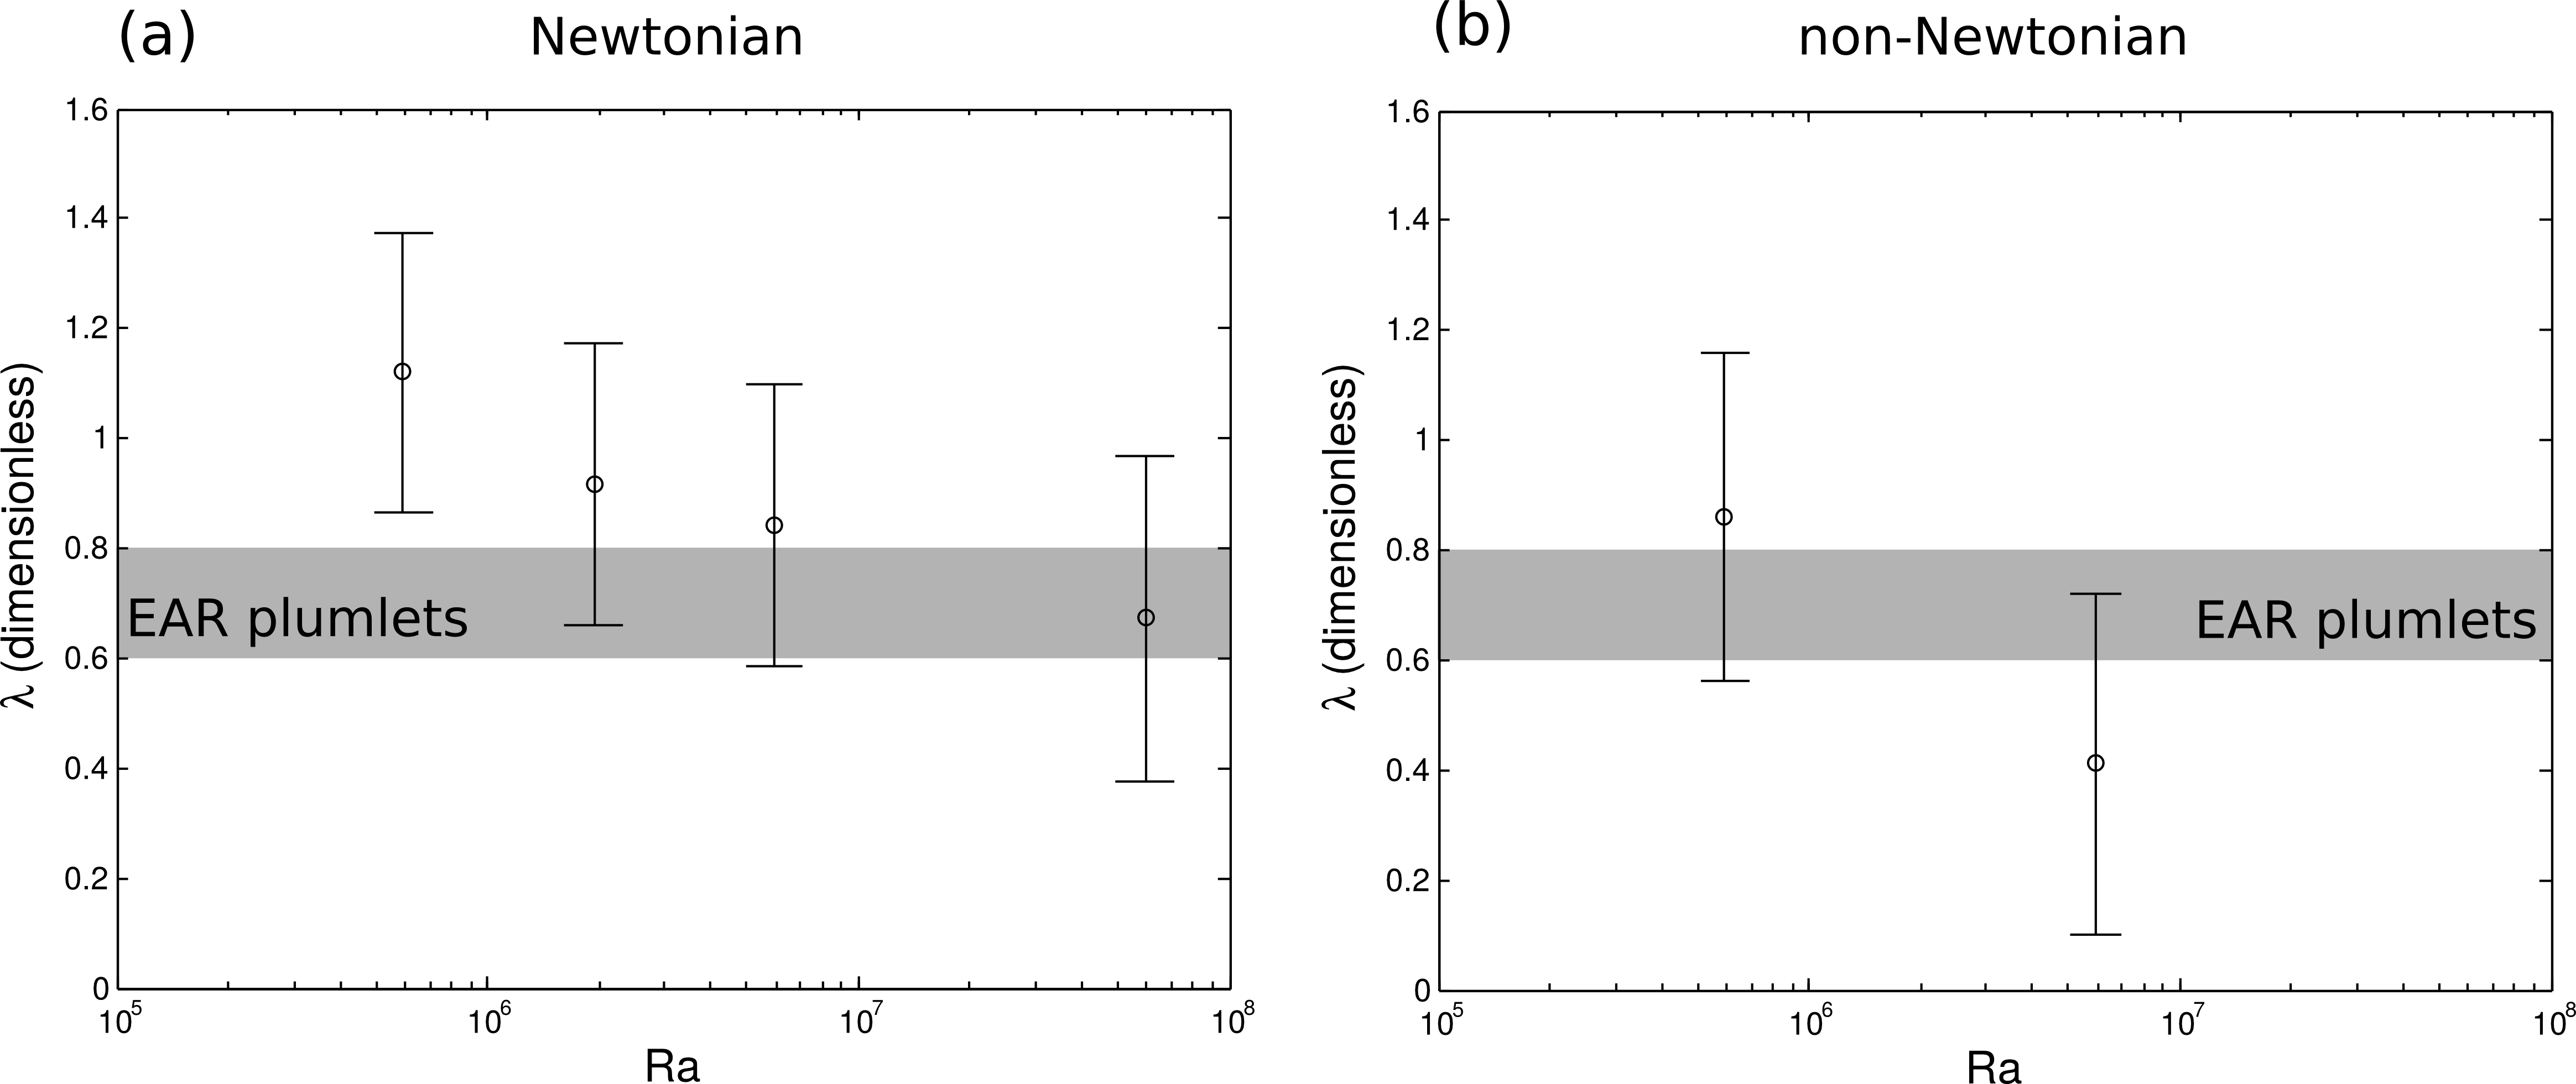
\includegraphics[width=11cm]{../figures-working/wavelengths.png}
\caption{Dimensionless wavelength for Rayleigh B{\'e}nard convection as a function of Raleigh number. (a) Newtonian models, showing the classic power law dependence between wavelength and Ra. The grey shaded area shows the estimate for the wavelength of the slow Vs anomalies below EAR, made dimensionless by dividing by the depth to the 660\,km depth seismic discontinuity. If these instabilities are due to Raleigh B{\'e}nard convection, we would require a low viscosity (high $Ra$). (b) Non-Newtonain models, showing a stronger dependence on $Ra$. However in this case at $Ra>10^7$, the plumes become difficult to detect given the plume tails are very thin. If the upper mantle is dominantly non-Newtonian, EAR plumlets are consistent with a higher viscosity (lower $Ra$).}
\label{fg:3}
\end{figure*}

For the Rayleigh B{\'e}nard experiments the model generates regularly spaced plumes for both the Newtonian and non-Newtonian rheologies (Fig.~\ref{fg:2}). These plumes grow uniformly across the model domain and the spacing is a function of the initial $Ra$ (Fig.~\ref{fg:3}). For the temperature dependent Newtonian rheology (models N1 to N4; Table \ref{tb:2}), rather classic mushroom shaped plumes are generated (Fig.~\ref{fg:2}a). These plumes eventually impinge on the buoyant lithosphere. The non-Newtonian model plumes are significantly thinner, with plume heads that rapidly flatten out under the lithosphere (Fig.\ref{fg:2}b). Using the definition of \cite{labrosse-2002} for finding the plume wavelength, we search for the distance between temperature anomalies of ,
\begin{equation}
T > \bar{T} + f\left(T_{max}- T_{min}\right)
\end{equation}
where $\bar{T}$ is the mean temperature, $T_{max}$ is maximum temperature, $T_{min}$ is the minimum temperature, and $f=0.2$. As in previous studies, we find that the wavelength of the plumes is a function of the $Ra$ number \citep{zhong-2005,galsa-2007,androvandi-etal-2011}. The trend in reduction in wavelength follows $\lambda/H \propto Ra^{1/6}$, however given the range in measured wavelengths we cannot rule out the possibility that $\lambda/H \propto Ra^{1/3}$, as found for laboratory experiments using fluids with a strongly temperature dependent viscosity (\citealp{androvandi-etal-2011}; Fig.~\ref{fg:3}a). The two data points for the non-Newtonian rheology (models N5 and N6) would suggest a stronger dependence of wavelength on $Ra$ when compared to the Newtonian models (Fig.~\ref{fg:3}b). Unfortunately, plumes at higher $Ra > 6\times10^{6}$ were too thin to be detected.

If we scale the dimensionless wavelength by the depth to the 660\,km depth seismic discontinuity we find that the possible EAR plumelets could be explained by Newtonian plumes with an upper mantle of $Ra > 10^6$ (Fig.~\ref{fg:3}a). This corresponds to a scaling viscosity, $\eta_{0} < 5\times10^{20}\rm\,Pa\,s$. For non-Newtonian plumes the wavelength of EAR plumelets corresponds to a $Ra$ for the upper mantle of $\sim 10^6$, or a reference viscosity of $\eta_{0} < 5\times10^{20}\rm\,Pa\,s$. However, these plumes are very likely too thin to be seismically visible.

\begin{figure*}
\centering
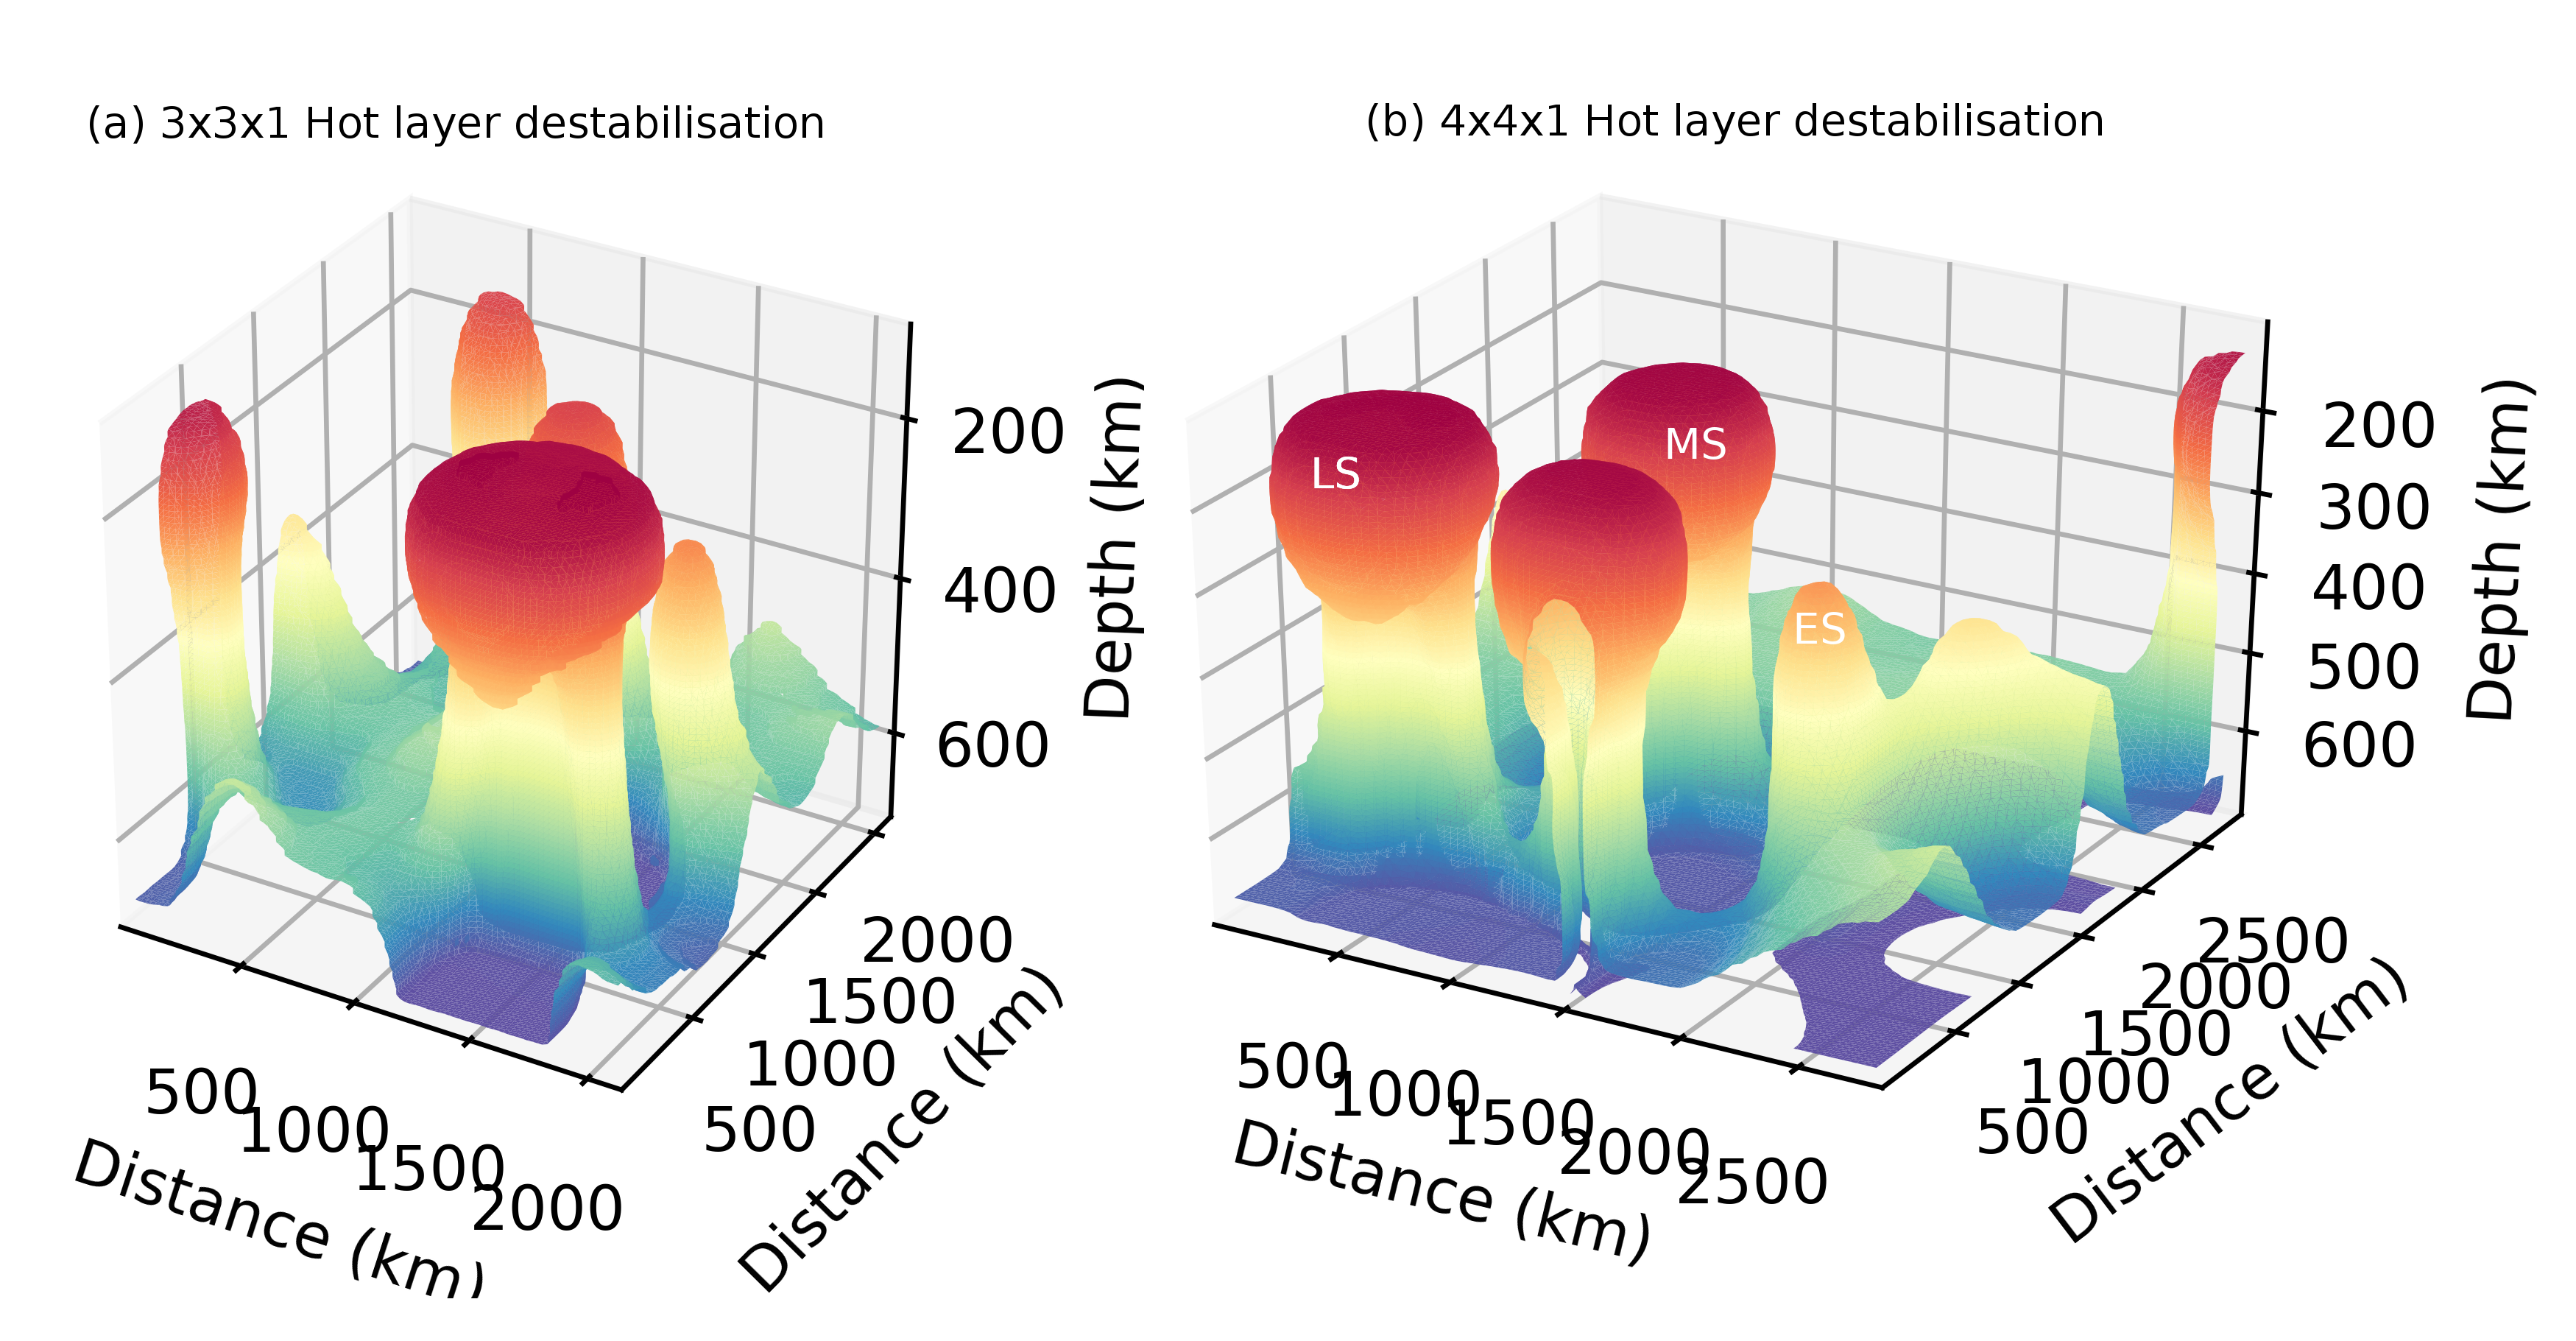
\includegraphics[width=16cm]{../figures-working/comparison-3x4-lables.png}
\caption{Comparison of patterns of destabilisation of a $100\,^{\circ}$C hot layer for a 3x3x1 and 4x4x1 Cartesian box (models N7 and N8 in Table \ref{tb:2}). Labeled are ES - early stage plumelet; MS - mid-stage plumelet; and LS - late stage plumelet.}
\label{fg:4}
\end{figure*}

\begin{figure*}
\centering
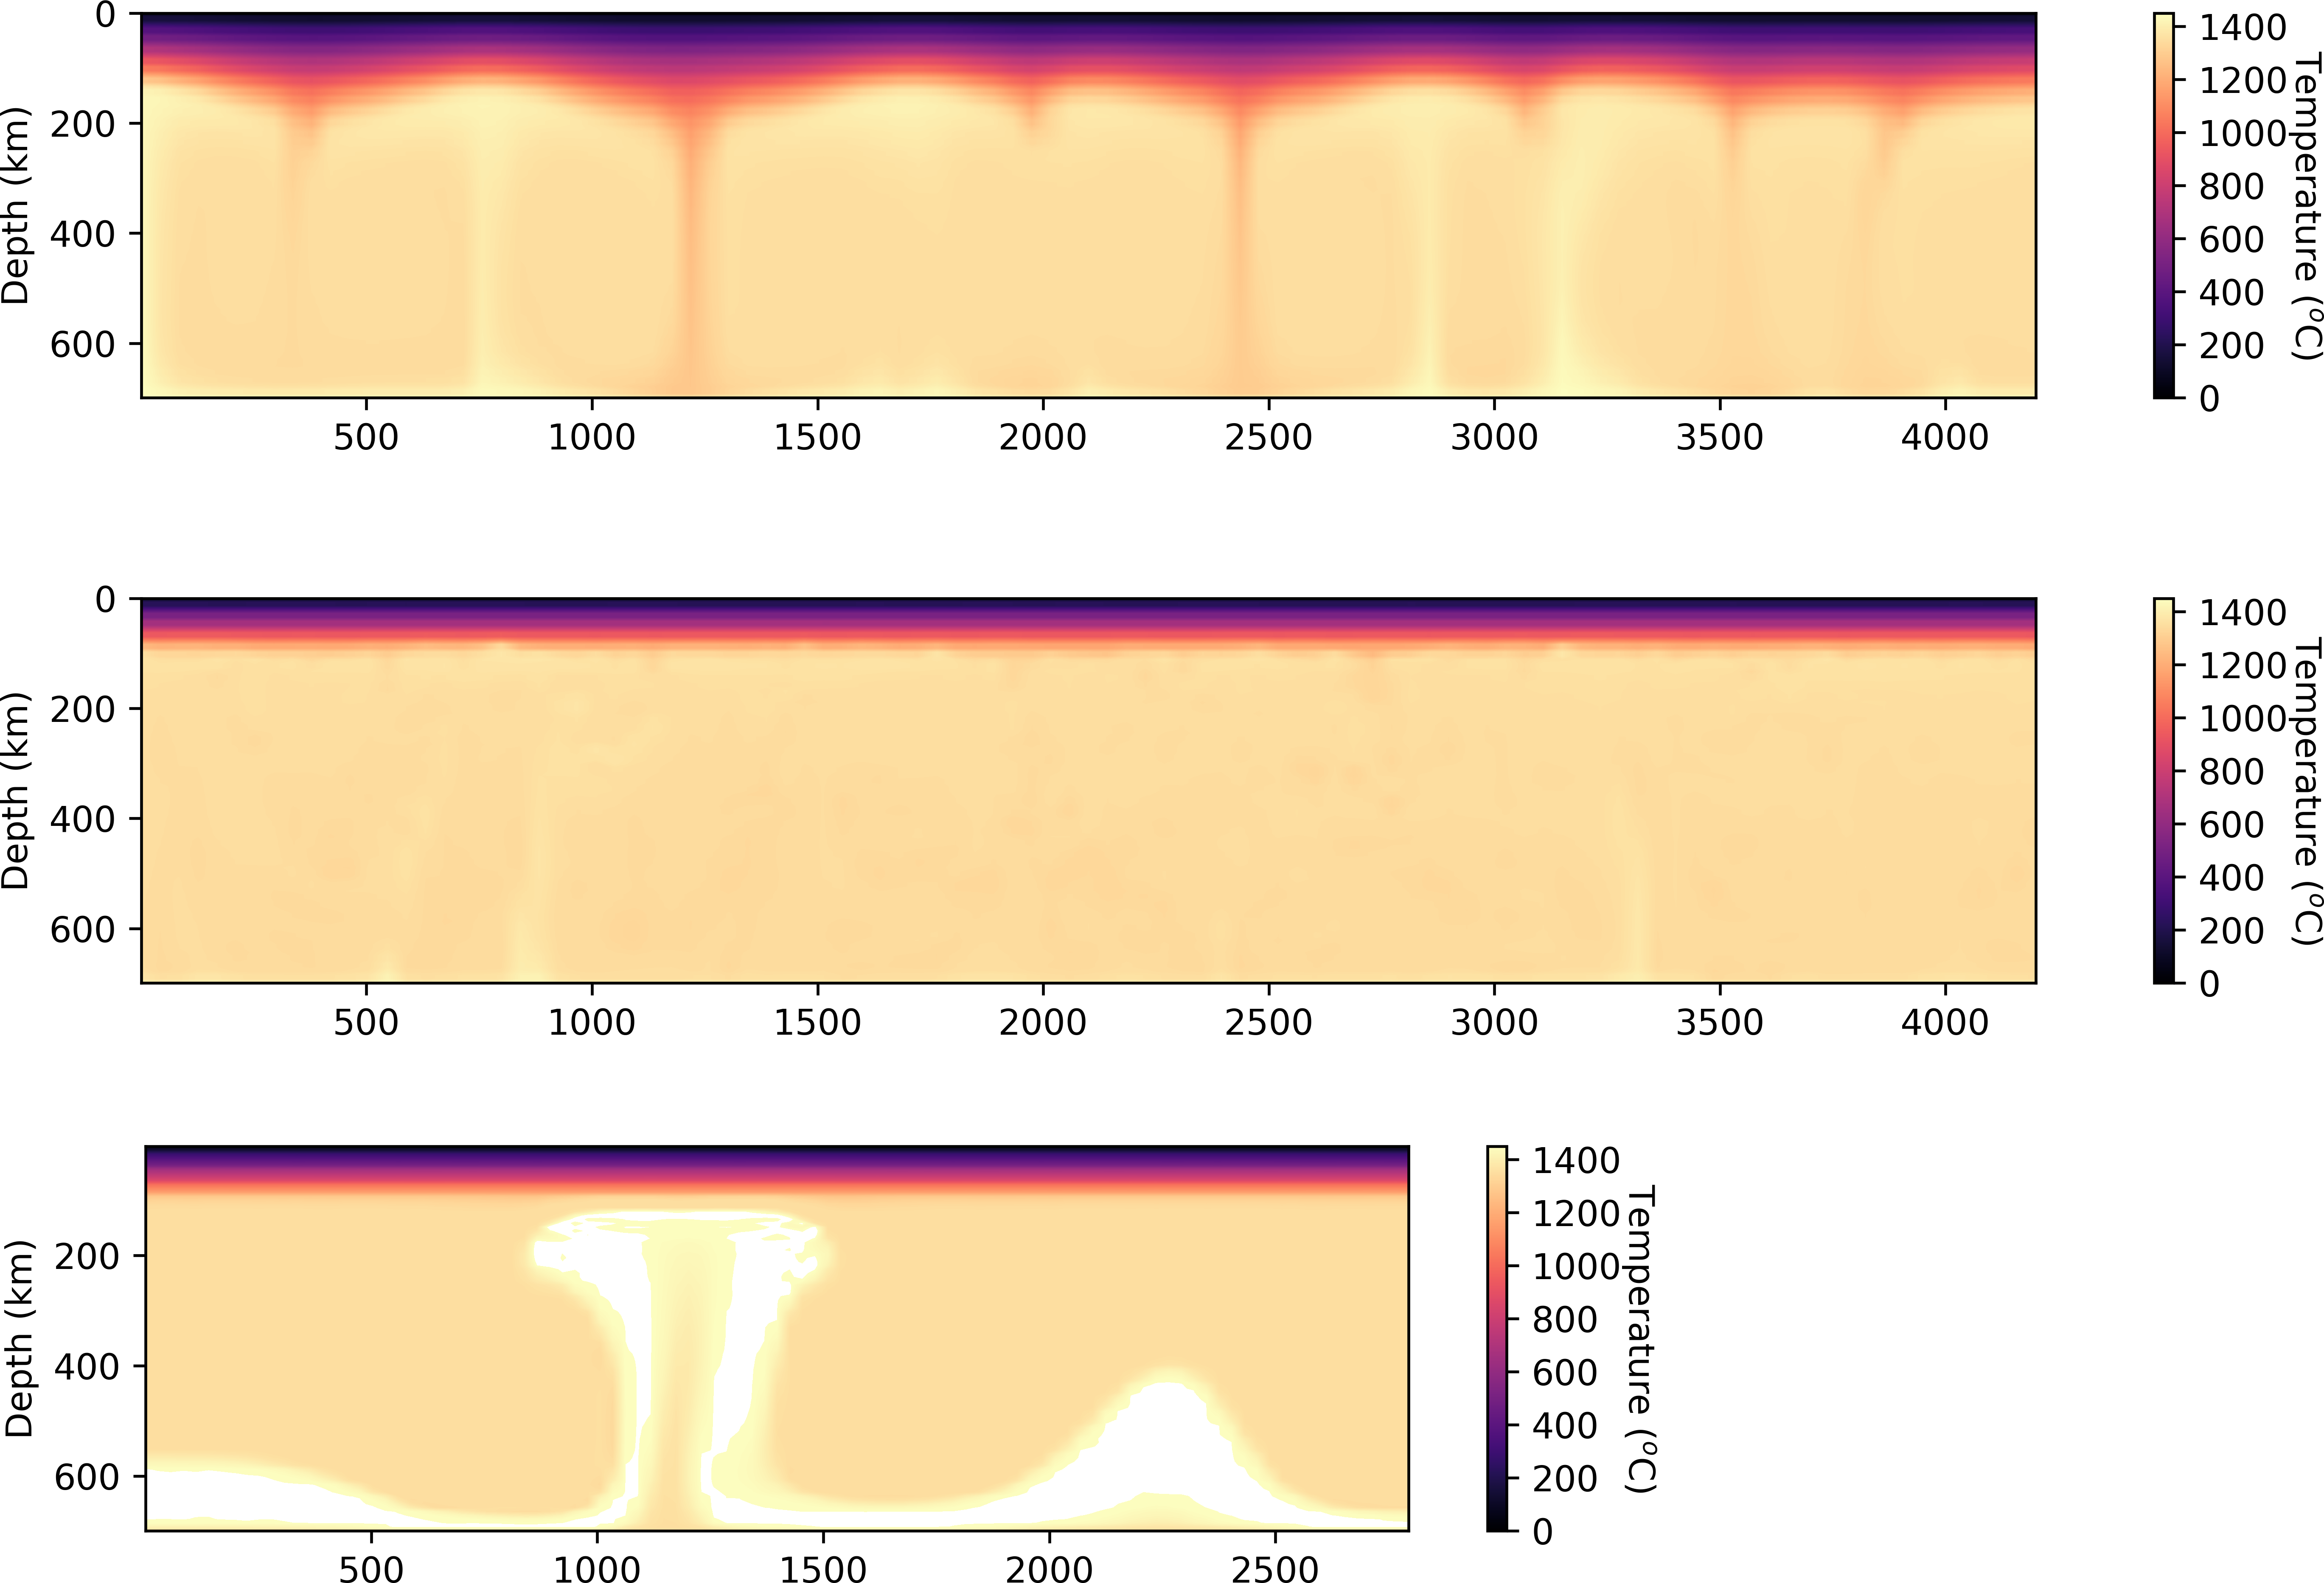
\includegraphics[width=11cm]{../figures-working/temperatures.png}
\caption{Cross section of Newtonian and non-Newtonian Rayleigh B{\'e}nard models N3 and N6 and the Rayleigh Taylor model N8.}
\label{fg:5}
\end{figure*}

The Rayleigh B{\'e}nard convection develops uniformly. The Rayleigh Taylor destabilisation of a hot layer of material is however not uniform in time (models N7 to N10; see Fig.~\ref{fg:4}). Here we can see early and late stage plume-like structures within the same snap-shot. The spacing of these instabilities is of the order $\lambda = 0.5H$ to $\lambda = H$ depending on the aspect ratio of the model domain and the stage at which the plume forms (Fig.~\ref{fg:4}; see models N7 and N8). The first instability always forms at a corner of the model, and this subsequently leads to a destabilization of the hot layer that propagates outwards form the corner. The wavelength of the plume-like structures was found to be independent of the temperature of the hot layer, as this did not significantly affect the initial $Ra$ number. Furthermore, the contrast in temperature is high for these plumes when compared to the Newtonian Rayleigh B{\'e}nard convection (Fig.~\ref{fg:5}). The strong temperature contrast is likely important.

When calculated seismic structures are converted to synthetic tomography the inverted magnitude of $V_{S}$ or $V_{P}$ diminishes \citep[e.g.][]{goes-etal-2012,maguire-etal-2018}. Therefore a strong temperature contrast might be required to match the significantly low seismic velocities inverted for below Afar and the MER (Figure \ref{fg:1}). This would suggest the Rayleigh Taylor structures would more likely correspond to the observed tomography. The wavelength of the plumelet spacing is however in this case dependent on the model aspect ratio. For the mode N7 (3x3x1) the spacing between rising plumelets is close to 800\,km when scaled to the upper mantle. For models N8 through to N10 the spacing is closer to 1000\,km (Fig.~\ref{fg:4}). Given that the Rayleigh Taylor plumelets can match the observed spacing and have a stronger temperature contrast we will explore how they are transformed when viewed as seismic anomalies.

\section{Synthetic tomography methods}

\subsection{Conversion to seismic anomalies}

To convert the thermal plume structures into velocities and density we follow the approach of \cite{cobden-etal-2008} and \cite{styles-etal-2011}. We use the thermo-dynamic code PerPlex \citep{connolly-2005} with the NCFMAS data base ‘stx08’ \citep{xu-etal-2008} to calculate the elastic parameters (bulk modulus $K$ and shear modulus $G$) and density as a function of pressure, temperature and composition. For the basic conversions, we assume a pyrolite composition, except for the continental lithosphere which is taken to be harzburgitic (both compositions from \citealp{xu-etal-2008}). A constant adiabatic temperature gradient of $0.45\rm\,K\,km^{-1}$ (a reasonable upper mantle average, according to \citealp{styles-etal-2011}) is added to the potential temperatures from the Boussinesq model. The velocities have further been corrected for the effects of temperature-, pressure-, and hydration dependent anelasticity using composite model $Q_{g}$ \citep{goes-etal-2012,vanwijk-etal-2008} for a frequency of 1\,Hz (which is good for the P-waves, but on the high side for the S-waves). The mantle is assumed to be damp (1000\,H/Si) and the continental lithosphere dry (50\,H/Si). The uncertainties involved in the calculation of elastic and anelastic parameters lead to uncertainties in $V_{P}$ and $V_{S}$ anomalies of around $\pm0.1$\,\% and $\pm 0.15$\,\%, respectively \citep{cammarano-etal-2003,styles-etal-2011}.

\begin{figure*}
\centering
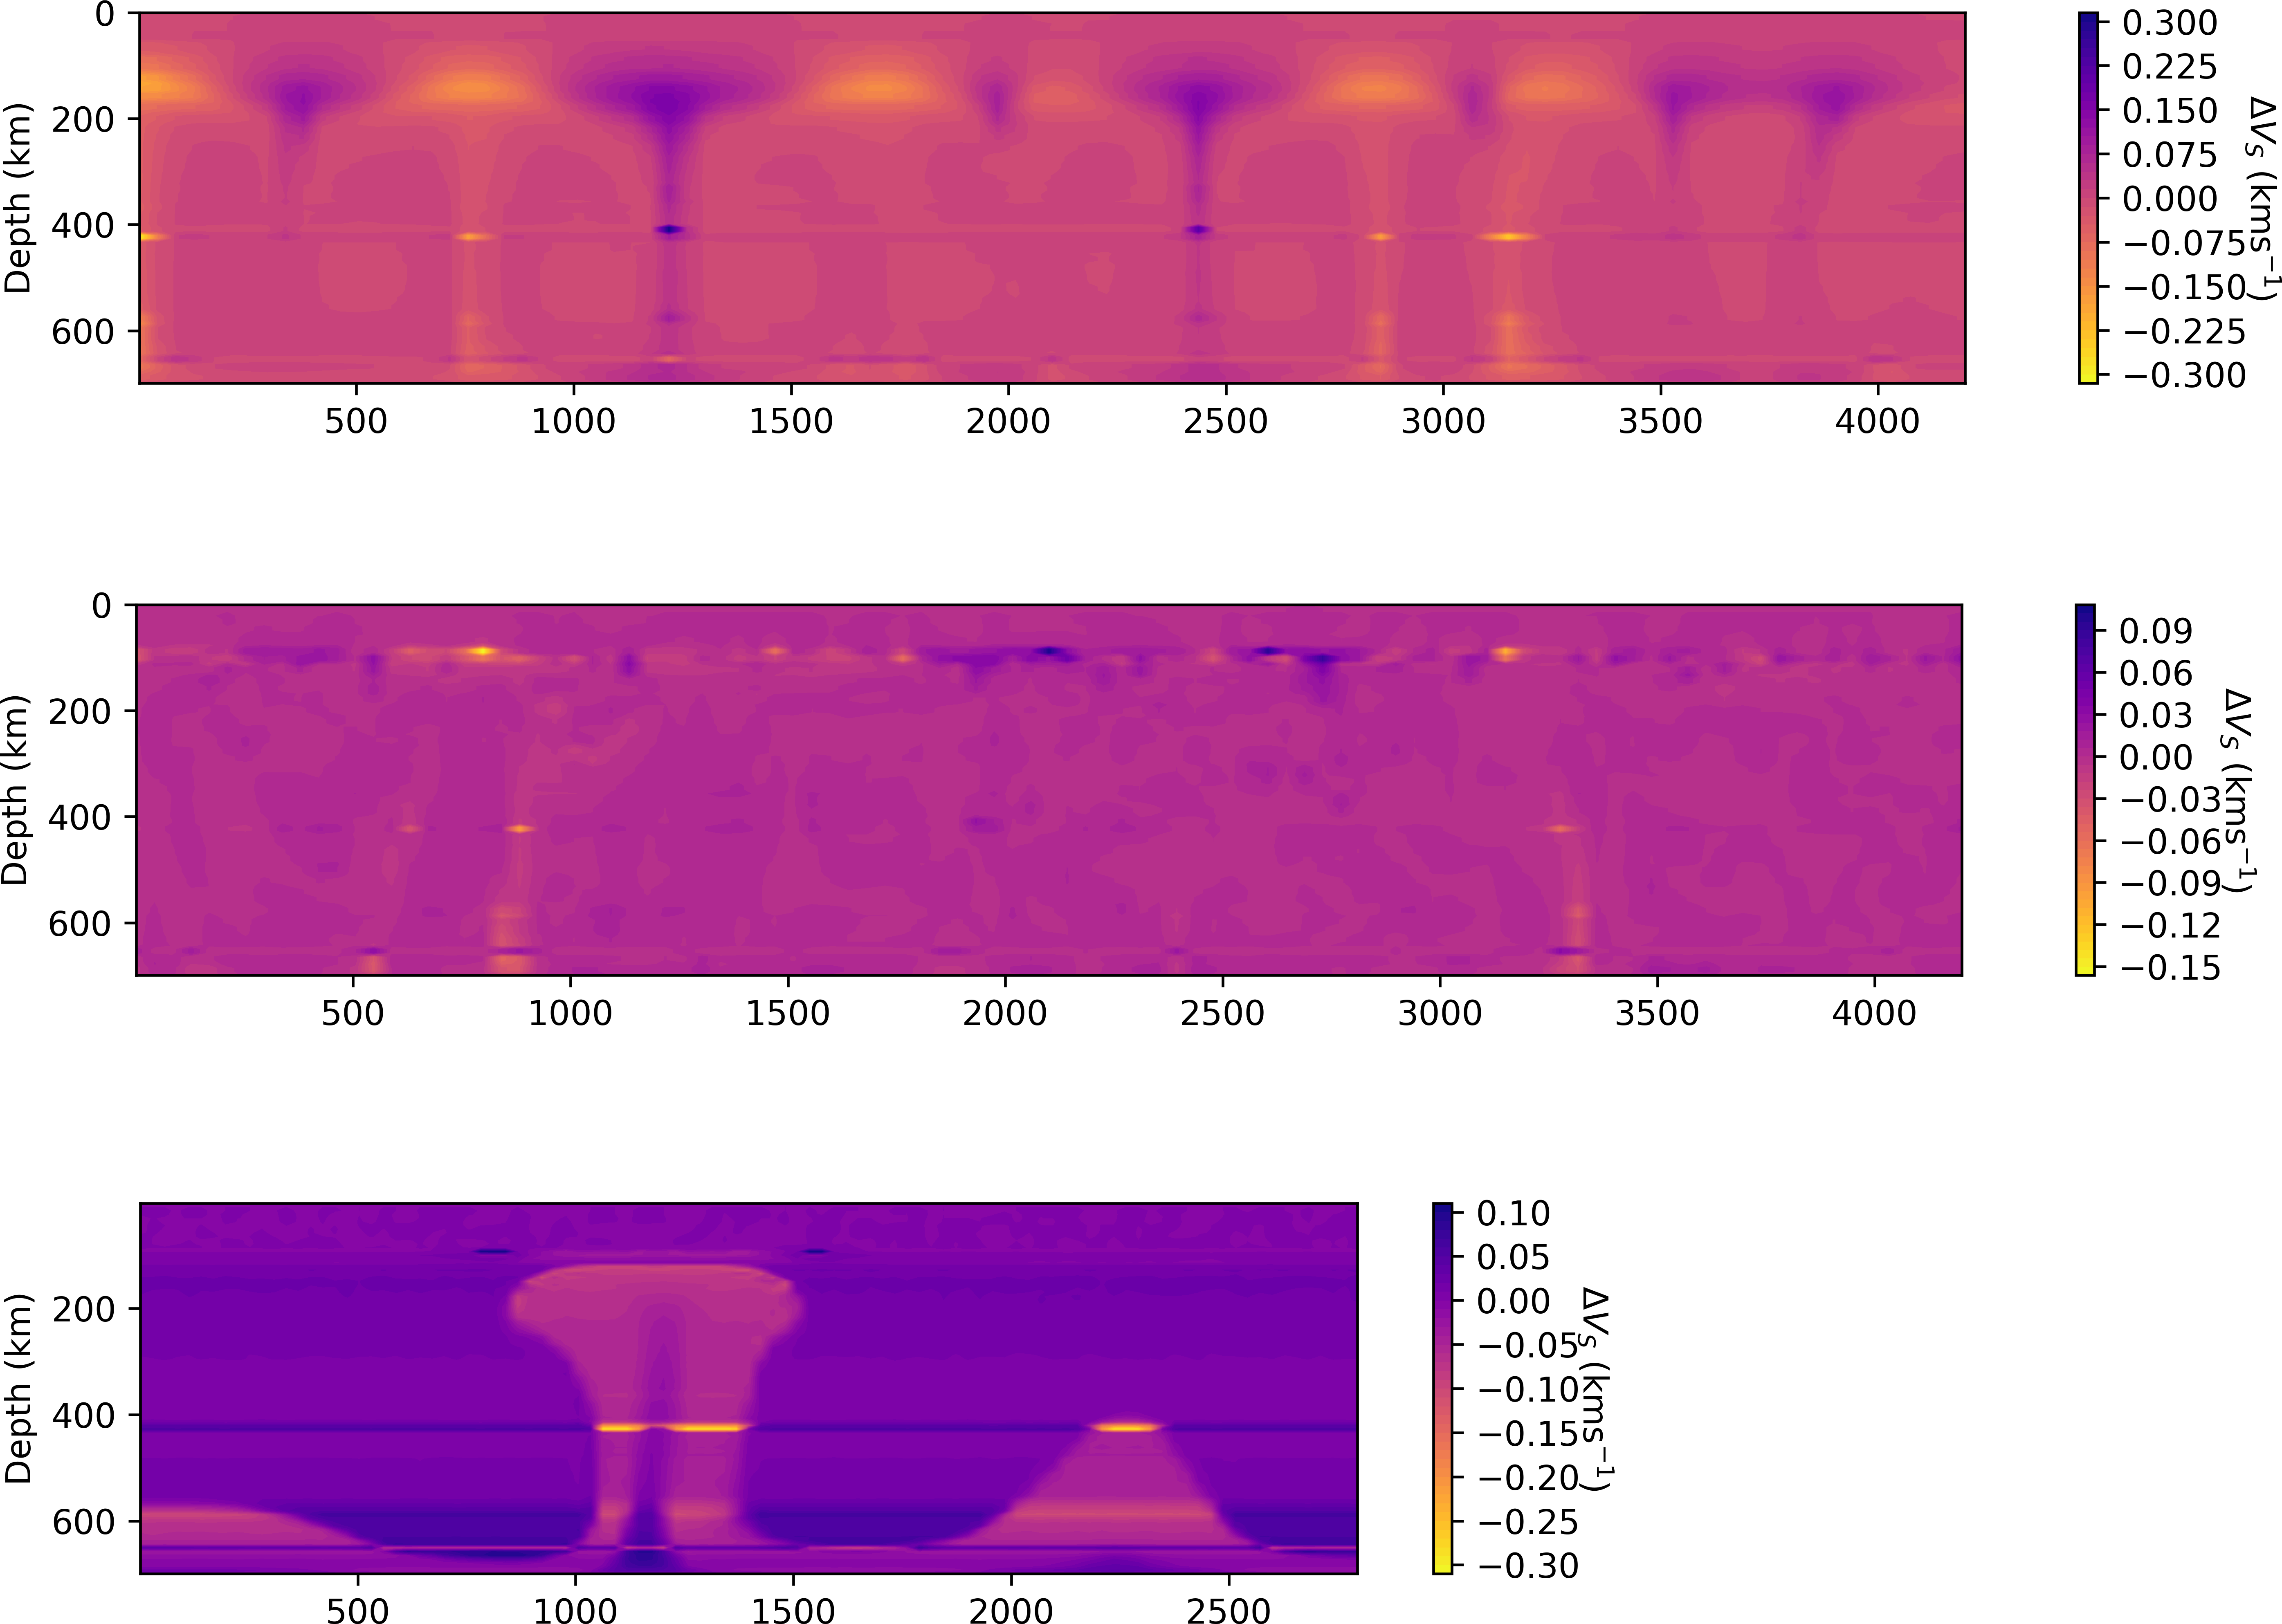
\includegraphics[width=11cm]{../figures-working/velocities.png}
\caption{Cross section of the S-wave seismic velocity anomaly relative to the horizontally averaged velocity for the Newtonian and non-Newtonian Rayleigh B{\'e}nard models N3 and N6 and the Rayleigh Taylor model N8.}
\label{fg:5b}
\end{figure*}

The plumelets can be seen in the seismic velocity anomalies to varying degrees depending on the model rheology and if they are due to Rayleigh B{\'e}nard convection (models N1 to N6; Fig.~\ref{fg:5b}a and b) or if  they form due to the destabilisation of a hot layer (models N7 to N10; Fig.~\ref{fg:5b}c). At shallow depths we also include the effect of melt. To include the basic effect of melt retention, we make a simple estimate of melt fractions and their signature: The dry solidus is approximated with a linear increase from $1100\,^{\circ}$C at 0\,km to $1700\,^{\circ}$C at 200\,km depth (based on the variation in the solidus from \citealp{herzberg-etal-2000}). Then we estimate a melt fraction from how much the actual (full) temperature exceeds the solidus, again using a linear relation where melt fraction is 0\,\% at the solidus temperature and reaches a maximum of 2\,\% for 300\,K excess temperature. We limit the range of melt fractions, assuming that melts are mobile and much larger melt fractions will escape rather than pool \citep[e.g.][]{faul-etal-1994}. To get the seismic anomalies due to melting, melt fractions are multiplied with the melt derivatives from \cite{hammond-2000}, which are -3.6 per percent melt volume for $V_{P}$ and -7.9 for $V_{S}$. This results in substantial local reductions in seismic wave speeds in the locations in the thermal structures where melt is expected.

\subsection{Tomographic method}

We test how the synthetic structure is imaged using the tomographic relative travel-time inversion for P- and S-wave velocity following the method of \cite{vandecar-etal-1995}. This technique cannot retrieve absolute velocities, but only anomalies relative to the average regional background. We perform a linear inversion and use ray theory which leaves some uncertainties in the determinations of the magnitude of the velocity anomaly, but should not change the overall anomaly patterns with depth \citep{montelli-etal-2004b}. We invert for these synthetic velocity structures using the same model parameterisation, regularisation scheme and parameters and raypaths (calculated through the iasp91 1D velocity model) as used in the tomography models of \cite{civiero-etal-2016,civiero-etal-2015}.

The synthetic datasets comprise 16420 relative P-wave arrival times and 16569 S-wave arrival times at 452 and 379 stations, respectively, for P- and S-wave travel times. We calculate the arrival times by applying full 3D ray tracing \citep{julian-1977} through the synthetic models and add Gaussian random noise to the synthetic data, respectively 0.07\,s and 0.37\,s for P- and S-wave data, i.e., of similar magnitude as the estimated errors in the real data.

The resolution in the shallower part of the upper mantle (0-200\,km depth) is low due to a lack of crossing rays at this depth range. In the inversion of seismic observationsthe 3D structure obtained from the surface-wave model of \cite{fishwick-2010} as an additional constraint on the shallow mantle structure \citep{civiero-etal-2016,civiero-etal-2015}. The P-wave speed starting model has been obtained converting the absolute shear velocities from the shear wave speeds to temperature and VP following \cite{goes-2002} and assuming that the S-wave anomalies were purely thermal in nature (see \citealp{civiero-etal-2015} for further details). To mimic this in the synthetic tomography, we moderately damp the model (damping $= 35$) towards the synthetic structure down to 350\,km. This is an optimistic test, as surface waves tomography will not retrieve the exact seismic structure; therefore, the damped version for the observed tomography is somewhere between the undamped and damped synthetic cases.

\begin{figure}
\centering
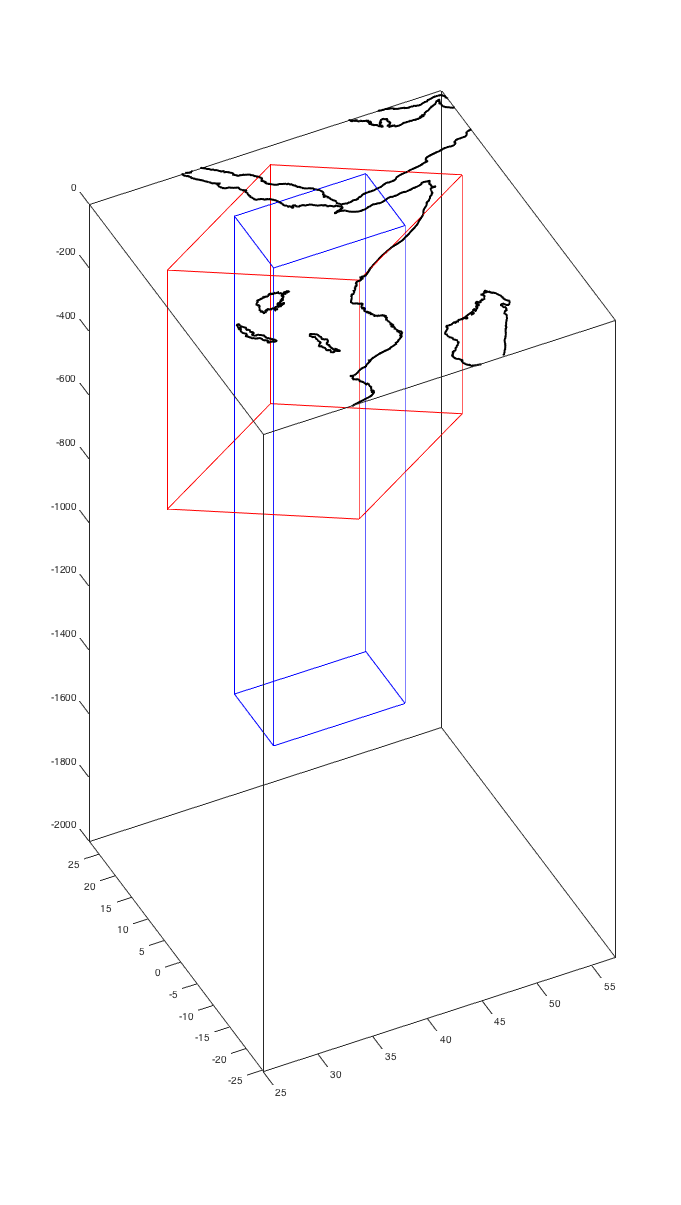
\includegraphics[width=8.6cm]{../figures-working/fig06.png}
\caption{3D perspective figure illustrating the relative sizes and locations of the tomographic and numerical model boxes. The black volume is the whole volume for the tomographic inversion. The red box is the volume of the numerical model used to perform the plume resolution tests, in this case rotated by $225^{\circ}$ with respect to the north direction. This orientation in space places the synthetic low-velocity structures at the same position as the imaged tomographic low-velocity anomalies beneath Afar and MER. The blue volume represents our region of interpretation, parameterised with a finer grid than outside.}
\label{fg:6}
\end{figure}

To perform the resolution tests, the numerical models need to be projected onto the tomographic grid. Because the tomographic grid is coarser than the numerical one, some of the finer scale features are not captured when the numerical model is re-sampled onto the tomographic grid. The volume of the whole tomographic model spans the range 28$^{\circ}$ N - 25.40$^{\circ}$S in latitude, 25$^{\circ}$E - 57.20$^{\circ}$E in longitude and 0-2000\,km in depth (shown by the black box in Fig.~\ref{fg:6}), with a node spacing respectively of 0.5$^{\circ}$, 0.4$^{\circ}$ and 50\,km. We focus our interpretation within the region (5–17$^{\circ}$N and 35–47$^{\circ}$E) comprising the Afar and MER regions (blue box in Fig.~\ref{fg:6}, area outlined in Fig.~\ref{fg:1}), where we have the highest density of crossing rays. The numerical model is a box of $19^{\circ} \times 19^{\circ}$ that extends from the surface up to $\sim800$\,km depth (red box in Fig.~\ref{fg:6}). Depending on the features we analyse, we rotate the model to position the different synthetic plume anomalies in the approximate locations of the two main low-velocity anomalies found in the observed P- and S-wave tomography, below Afar and west of the MER.

\section{Synthetic tomography results}

We focus on the Rayleigh Taylor instabilities given they have a strong temperature contrast (Fig. \ref{fg:5}), and have a wavelength that is similar to that interpreted form the tomographic observations. We will explore both models with an aspect ratio of 3x3x1 (model N7) and 4x4x1 (models N8 to N10; Table \ref{tb:2}). The increased numerical resolution of models N8 to N10 allowed us to model very large temperatures contrasts between the asthenosphere and the plumelet temperatures, 100 to $400\rm\,^{\circ}C$ (Table \ref{tb:2}).

\subsection{Plume resolution}

\begin{figure*}
\centering
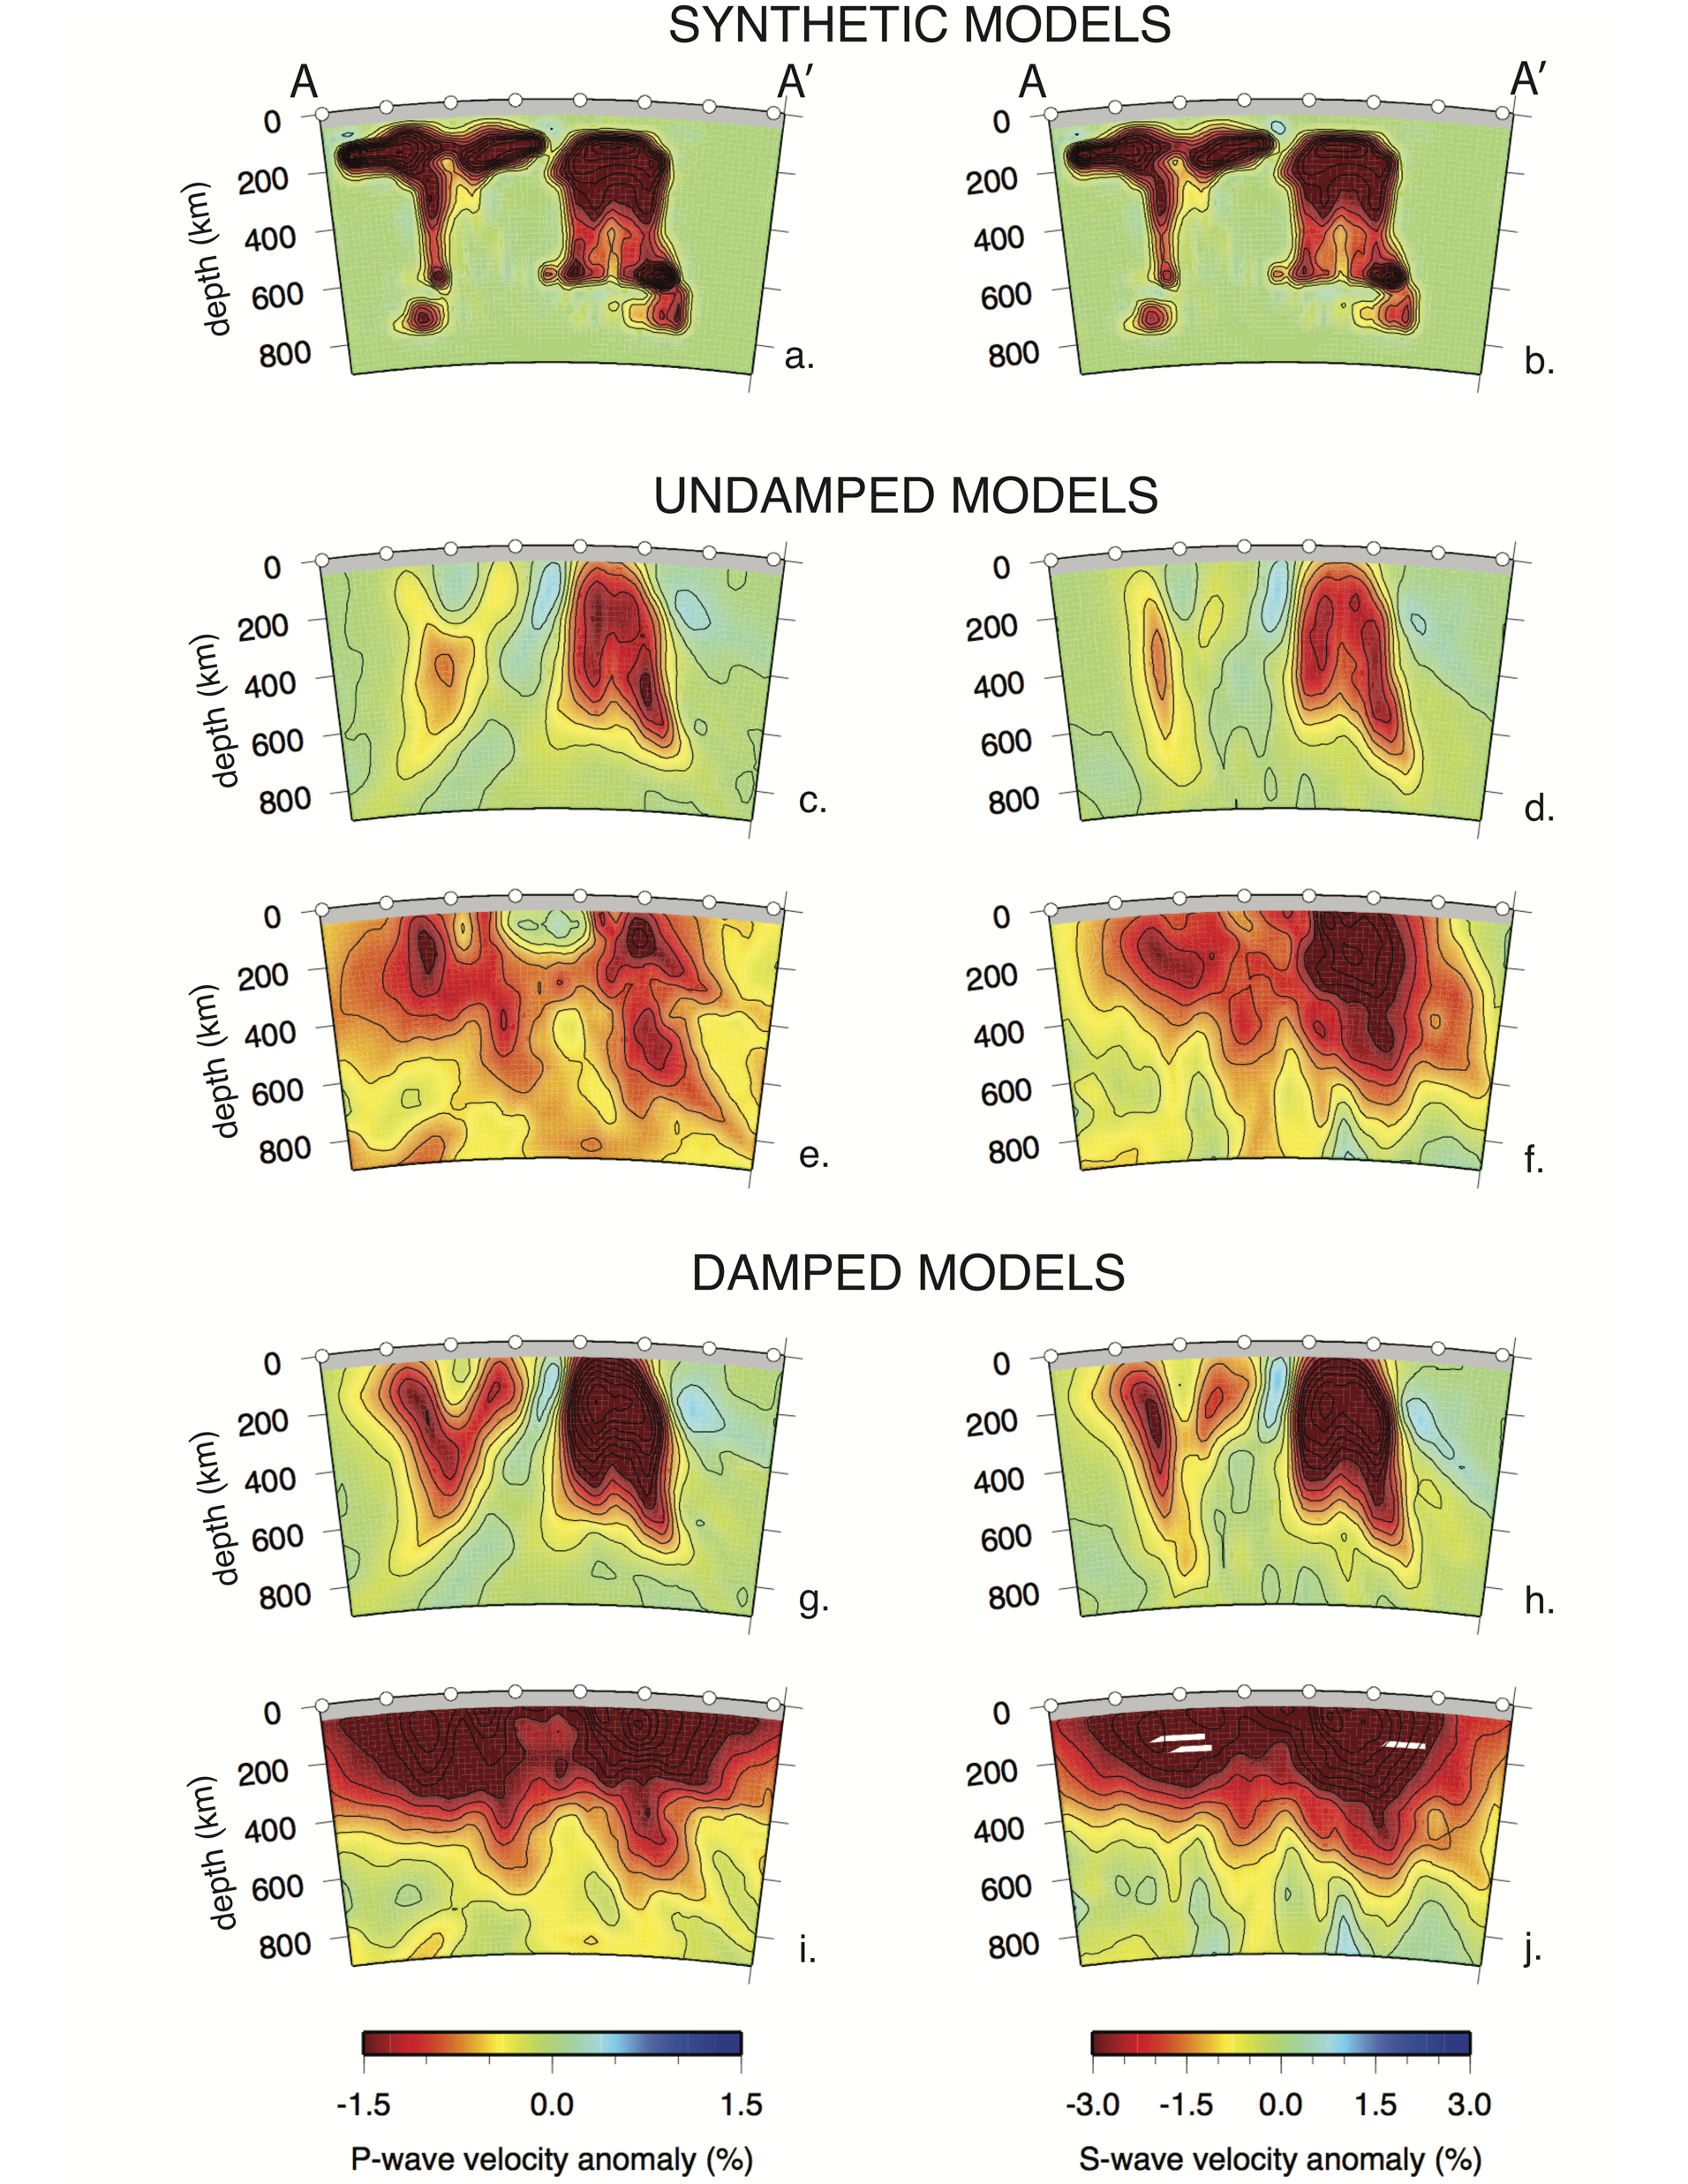
\includegraphics[width=11cm]{../figures-working/fig07.png}
\caption{(a) P-wave velocity anomalies (\%) along a vertical cross-section through the input model N7 oriented such that the two plumes shown are positioned approximately under Afar and west of the MER. (b) Input S-wave velocity anomaly (\%). The location of the cross-sections (black line) is shown in Fig.~\ref{fg:1}b. The structure on the right represents the synthetic middle-stage (MS) plume, the structure on the left the late-stage (LS) plume discussed in the text. (c, d, g, h) Vertical cross-sections through the recovered undamped (damping $=0$) (c-d) P- (c) and S-wave (d) models and the moderately damped (damping $=35$) P- (g) and S-wave (h) models. e, i) Vertical cross-sections of the undamped (e) and damped (i) NEAR-P15 model. (f, j) Vertical cross-sections of the undamped (f) and damped (j) NEAR-S16 model. The spacing between the contours is 0.25\,\% for P-wave models and 0.50\,\% for S-wave models. White points indicate distance every $2^{\circ}$. Both the undamped models (c–d) and the damped recovered models (g–f) image most of the middle-stage plume, and only the head, but with relatively subdued amplitudes, of the late stage plume. The scale of the recovered structures is quite similar to that of imaged features.}
\label{fg:7}
\end{figure*}

We use the model N7 (see Table \ref{tb:2}) to illustrate the resolution of the synthetic plume structures below Afar and MER and compare the resolved models with the observed P- and S-wave tomography. We rotated the plume model in order to place a middle-stage plume with a broad head and a thick stem below Afar, a late-stage plume with a head spread at the base of the lithosphere, and a narrow tail below MER (Fig.~\ref{fg:7}a and b). Synthetic cross sections of the same orientation as the sections through models NEAR-P15 and NEAR-S16 in Fig.~\ref{fg:1} are shown in Fig.~\ref{fg:7}c, d, g, and h. The middle-stage plume located beneath Afar are generally well recovered, although details, such as a partially folded head and a tail influenced by phase-boundary topography are not identifiable. The anomalies from the late-stage upwelling below the MER are recovered less clearly, especially in the undamped case, where the plume head, which has spread along the base of the lithosphere, is not fully resolved (Fig.~\ref{fg:7}c, d). The recovery of the plume geometries can be enhanced if constraints on the shallow structure and damping towards it are added (Fig.~\ref{fg:7}g, h; see \citealp{civiero-etal-2016,civiero-etal-2015}). Resolution for the P- and S-wave models is visually very similar. Some of the differences between the recovery of the two plumes may be due to different resolution below Afar and MER as the data coverage is slightly higher in the first region than in the latter.

Although a Cartesian model of the destabilisation of a $100\,^{\circ}$C hot layer (model N8) cannot be expected to match the actual imaged structures in detail, the similarities between them are striking. The scale and spacing of the modelled plumes, after accounting for the seismic resolution, is similar to the observed features. Only the low velocities at shallow depths are not as
widespread in the synthetic tomography compared to the observed tomography (see Fig.~\ref{fg:7}g, h, i, j).

Interestingly, NEAR-P15 and NEAR-S16 have some differences in relative P-wave over S-wave anomaly amplitude and structure of the low-velocity anomalies below Afar and the MER (Fig.~\ref{fg:7}e, f, i, j; \citealp{civiero-etal-2016}). However, similar differences occur in the synthetic tests as well: The retrieved plume structure below Afar looks more pronounced in the S- than in the P-wave model, while the structure below MER looks more discontinuous in P-wave model than in the S-wave model (Fig.~\ref{fg:7}c, d, g, h). Although resolution is similarly good for the P- and S-wave models, small differences in spatial resolution due to the added lateral resolution supplied to the S-wave velocity inversion by the SKS-wave travel times leads to differences in the relative amplitudes of the imaged structures. This might mean that observed $V_{P}/V_{S}$ ratios represent differences in model resolution as well as possible effects due to for example melt within the asthenosphere.

\subsection{Plume temperature and geometry}

The model N7 has a remarkable similarity to the observed seismic tomography (Fig.~\ref{fg:7}). When the model aspect ratio is 3x3x1, the plumelet spacing is of the order of 800\,km and this allows us to rotate two plumes into a position that matches the two low seismic anomalies found below Afar and the MER. Models N8 to N10 have a wider plumelet spacing, due to their larger aspect ration, 4x4x1. This larger aspect ratio was chosen due to the requirement to have a larger numerical resolution to solve for the destabilisation of a hot layer with increased temperature, while efficiently spreading the numerical model across compute nodes. Therefor to test if a hotter thermal anomaly is required to match the seismic anomalies, we will explore how individual plumelets potentially match the observed tomography.

To test how the different plume temperatures, and plume geometries corresponding to different stages of plume evolution, might be resolved by travel-time tomography, we identify three distinct evolutionary phases for models N8 to N10 (labelled in Fig.~\ref{fg:3}b). The first is an early-stage plume (ES) that is ascending from the thermal boundary layer and penetrating into the upper mantle without a well-defined head. The second structure is a middle-stage plume (MS) with a thinner feeder column of $\sim 150$\,km diameter and a voluminous head, $\sim 500$\,km diameter, developing in the upper mantle and has not reached the surface yet. The third is a late-stage plume (LS), which shows the classical mushroom type structure with a head spreading at the base of the lithosphere, followed by a thinner tail.

\begin{figure*}
\centering
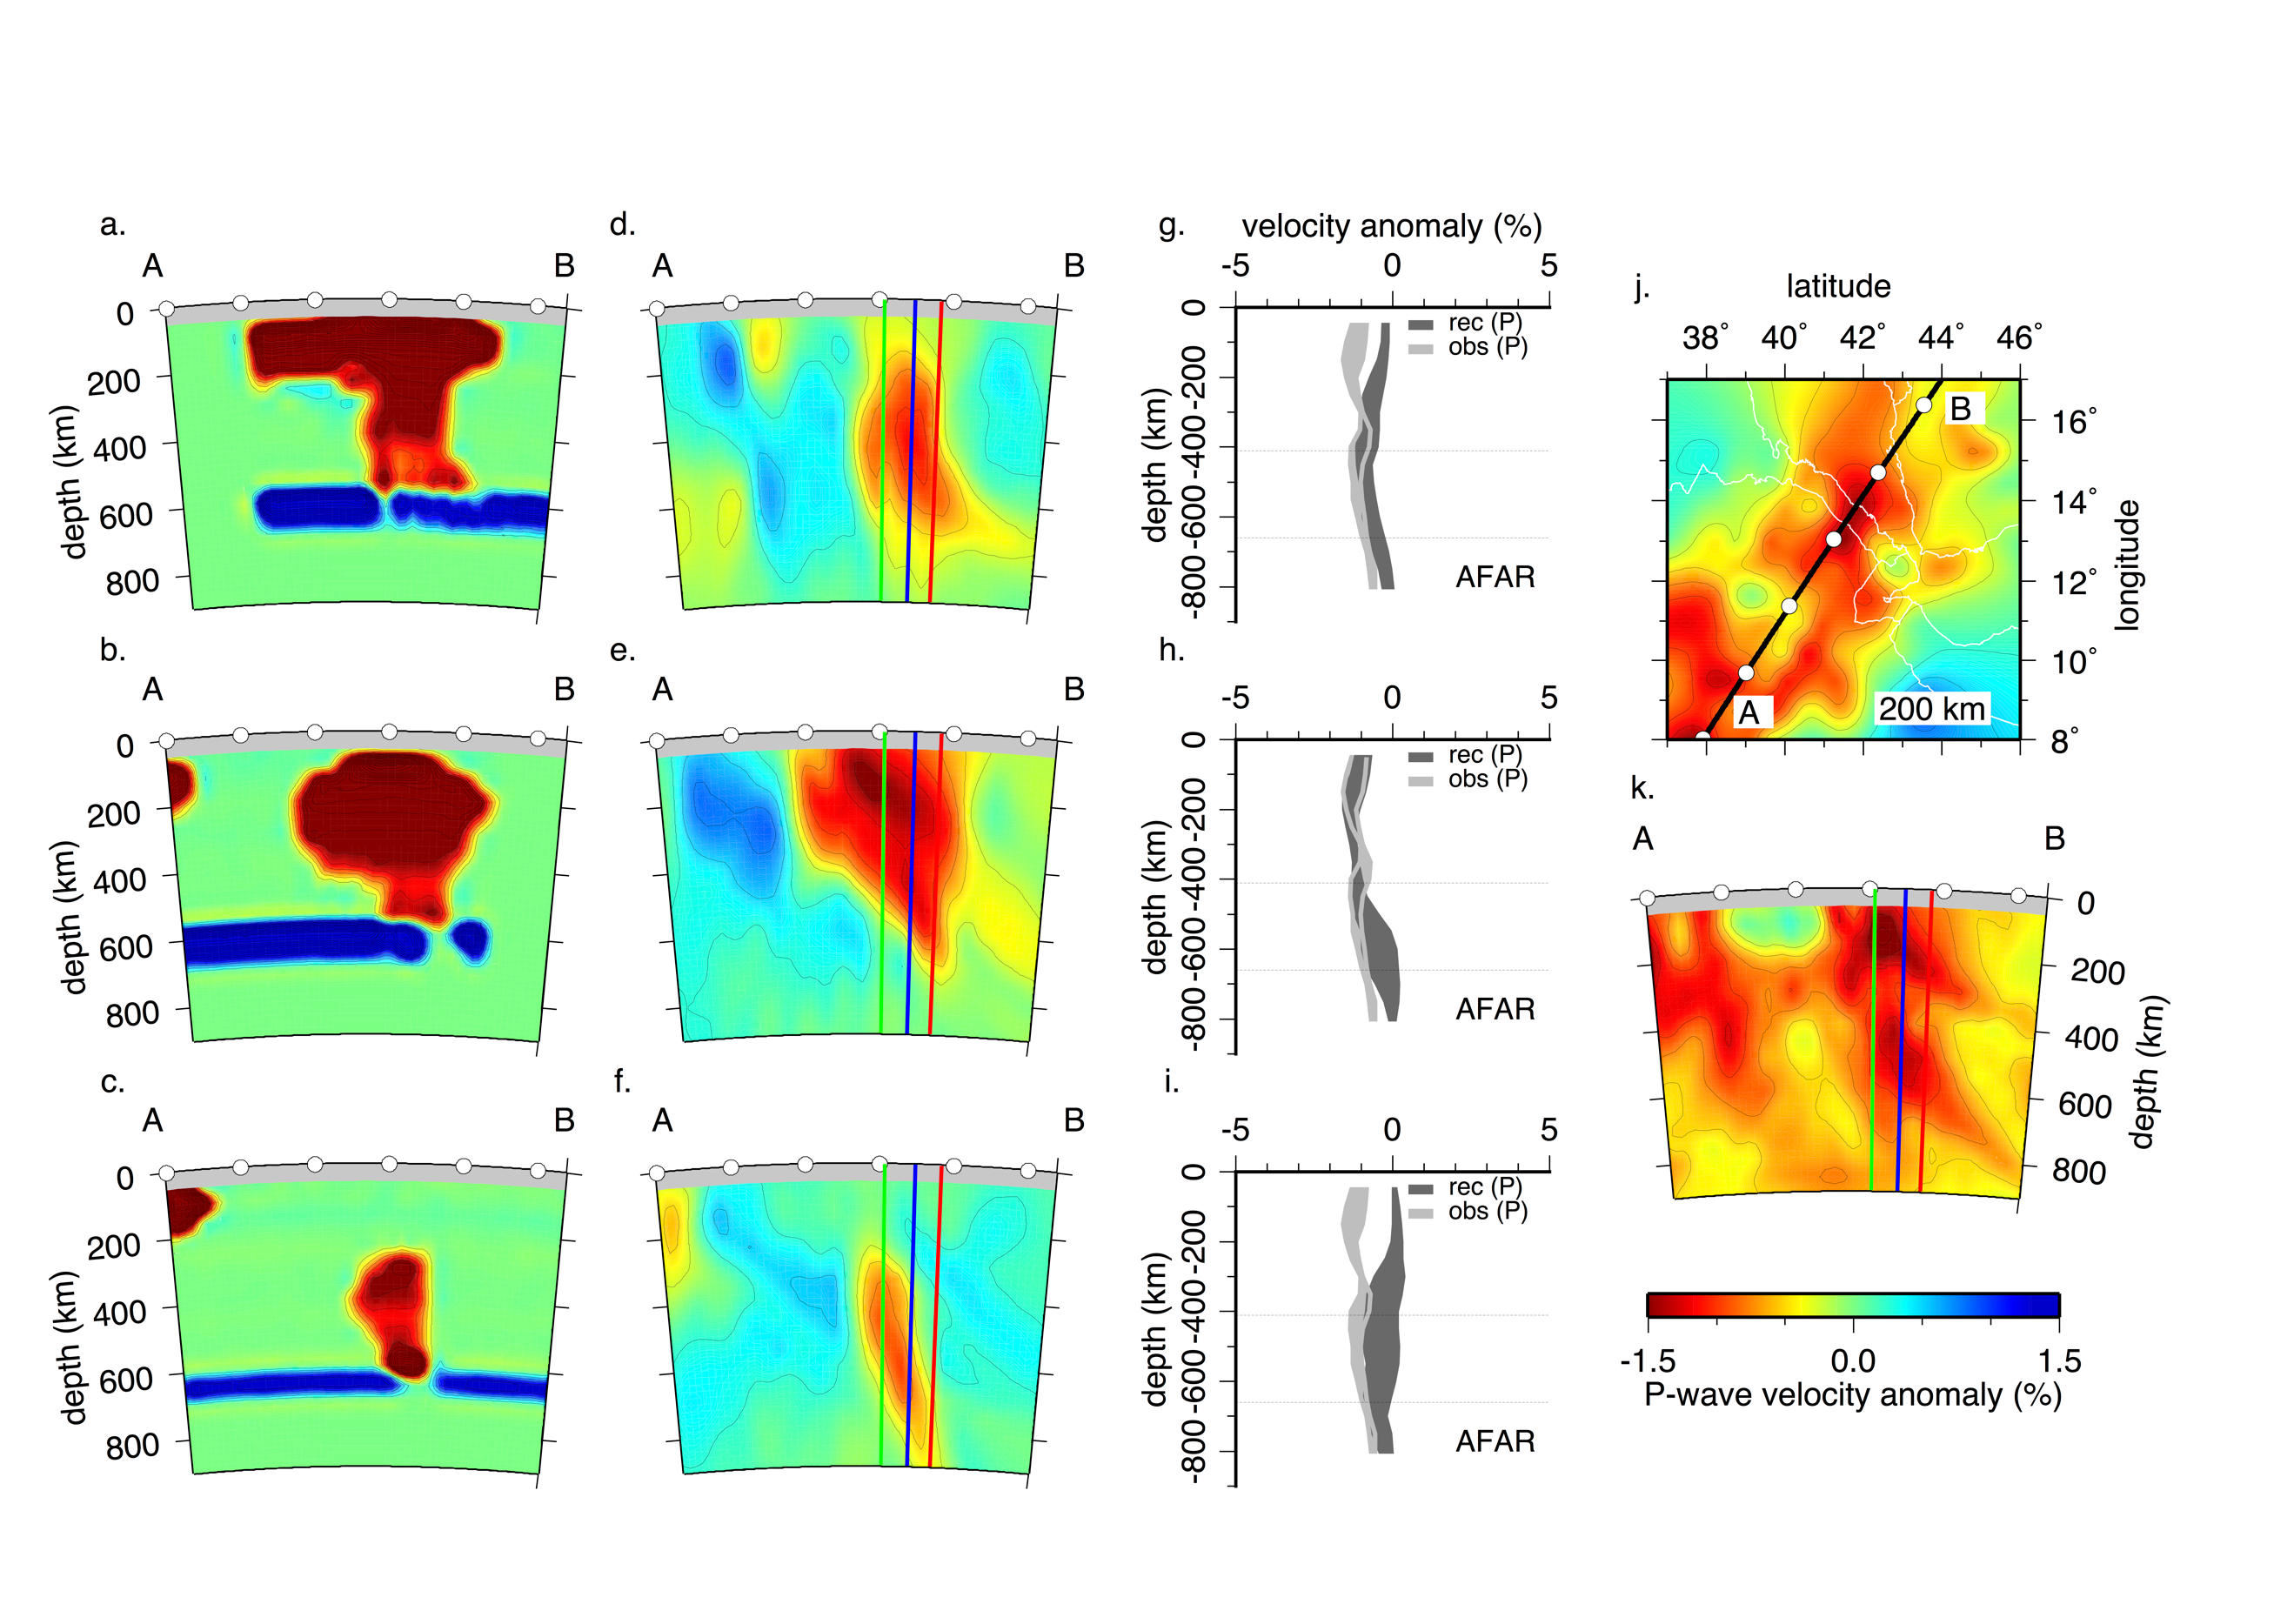
\includegraphics[width=16cm]{../figures-working/fig09.png}
\caption{Vertical cross-sections through the undamped P-wave model from model N9 with a $200\rm\,^{\circ}C$ hot layer, focused in the region below Afar.  The orientation of the cross-sections (black line) is shown in the 200 km depth slices through the NEAR-P15 tomographic model  j. (a, d) synthetic and resolved images of the LS phase of plume evolution; (b, e) synthetic and resolved images of the MS phase of plume evolution; (c-f) synthetic and resolved images of the ES phase of plume evolution. The imaged EP (g-j) and LP (i-l) phases are similar although the synthetic structures (a, c) are different due to the lack of resolution at shallow upper-mantle depths. The MS phase (e) is well resolved because the head of the input model (b) is relatively large. g-i) Input and retrieved P-wave velocity LS (g), MS (h) and ES (i) anomaly envelopes (\%) along the green, blue and red profiles drawn in the cross-sections. Within the transition zone the retrieved and observed velocity anomalies overlap. (j) 200 km depth slice through the undamped NEAR-P15 model k) Vertical cross-section of the undamped NEAR-P15 model. The spacing between the contours is 0.25\,\%. White points indicate the distance every $2^{\circ}$.}
\label{fg:8}
\end{figure*}

\begin{figure*}
\centering
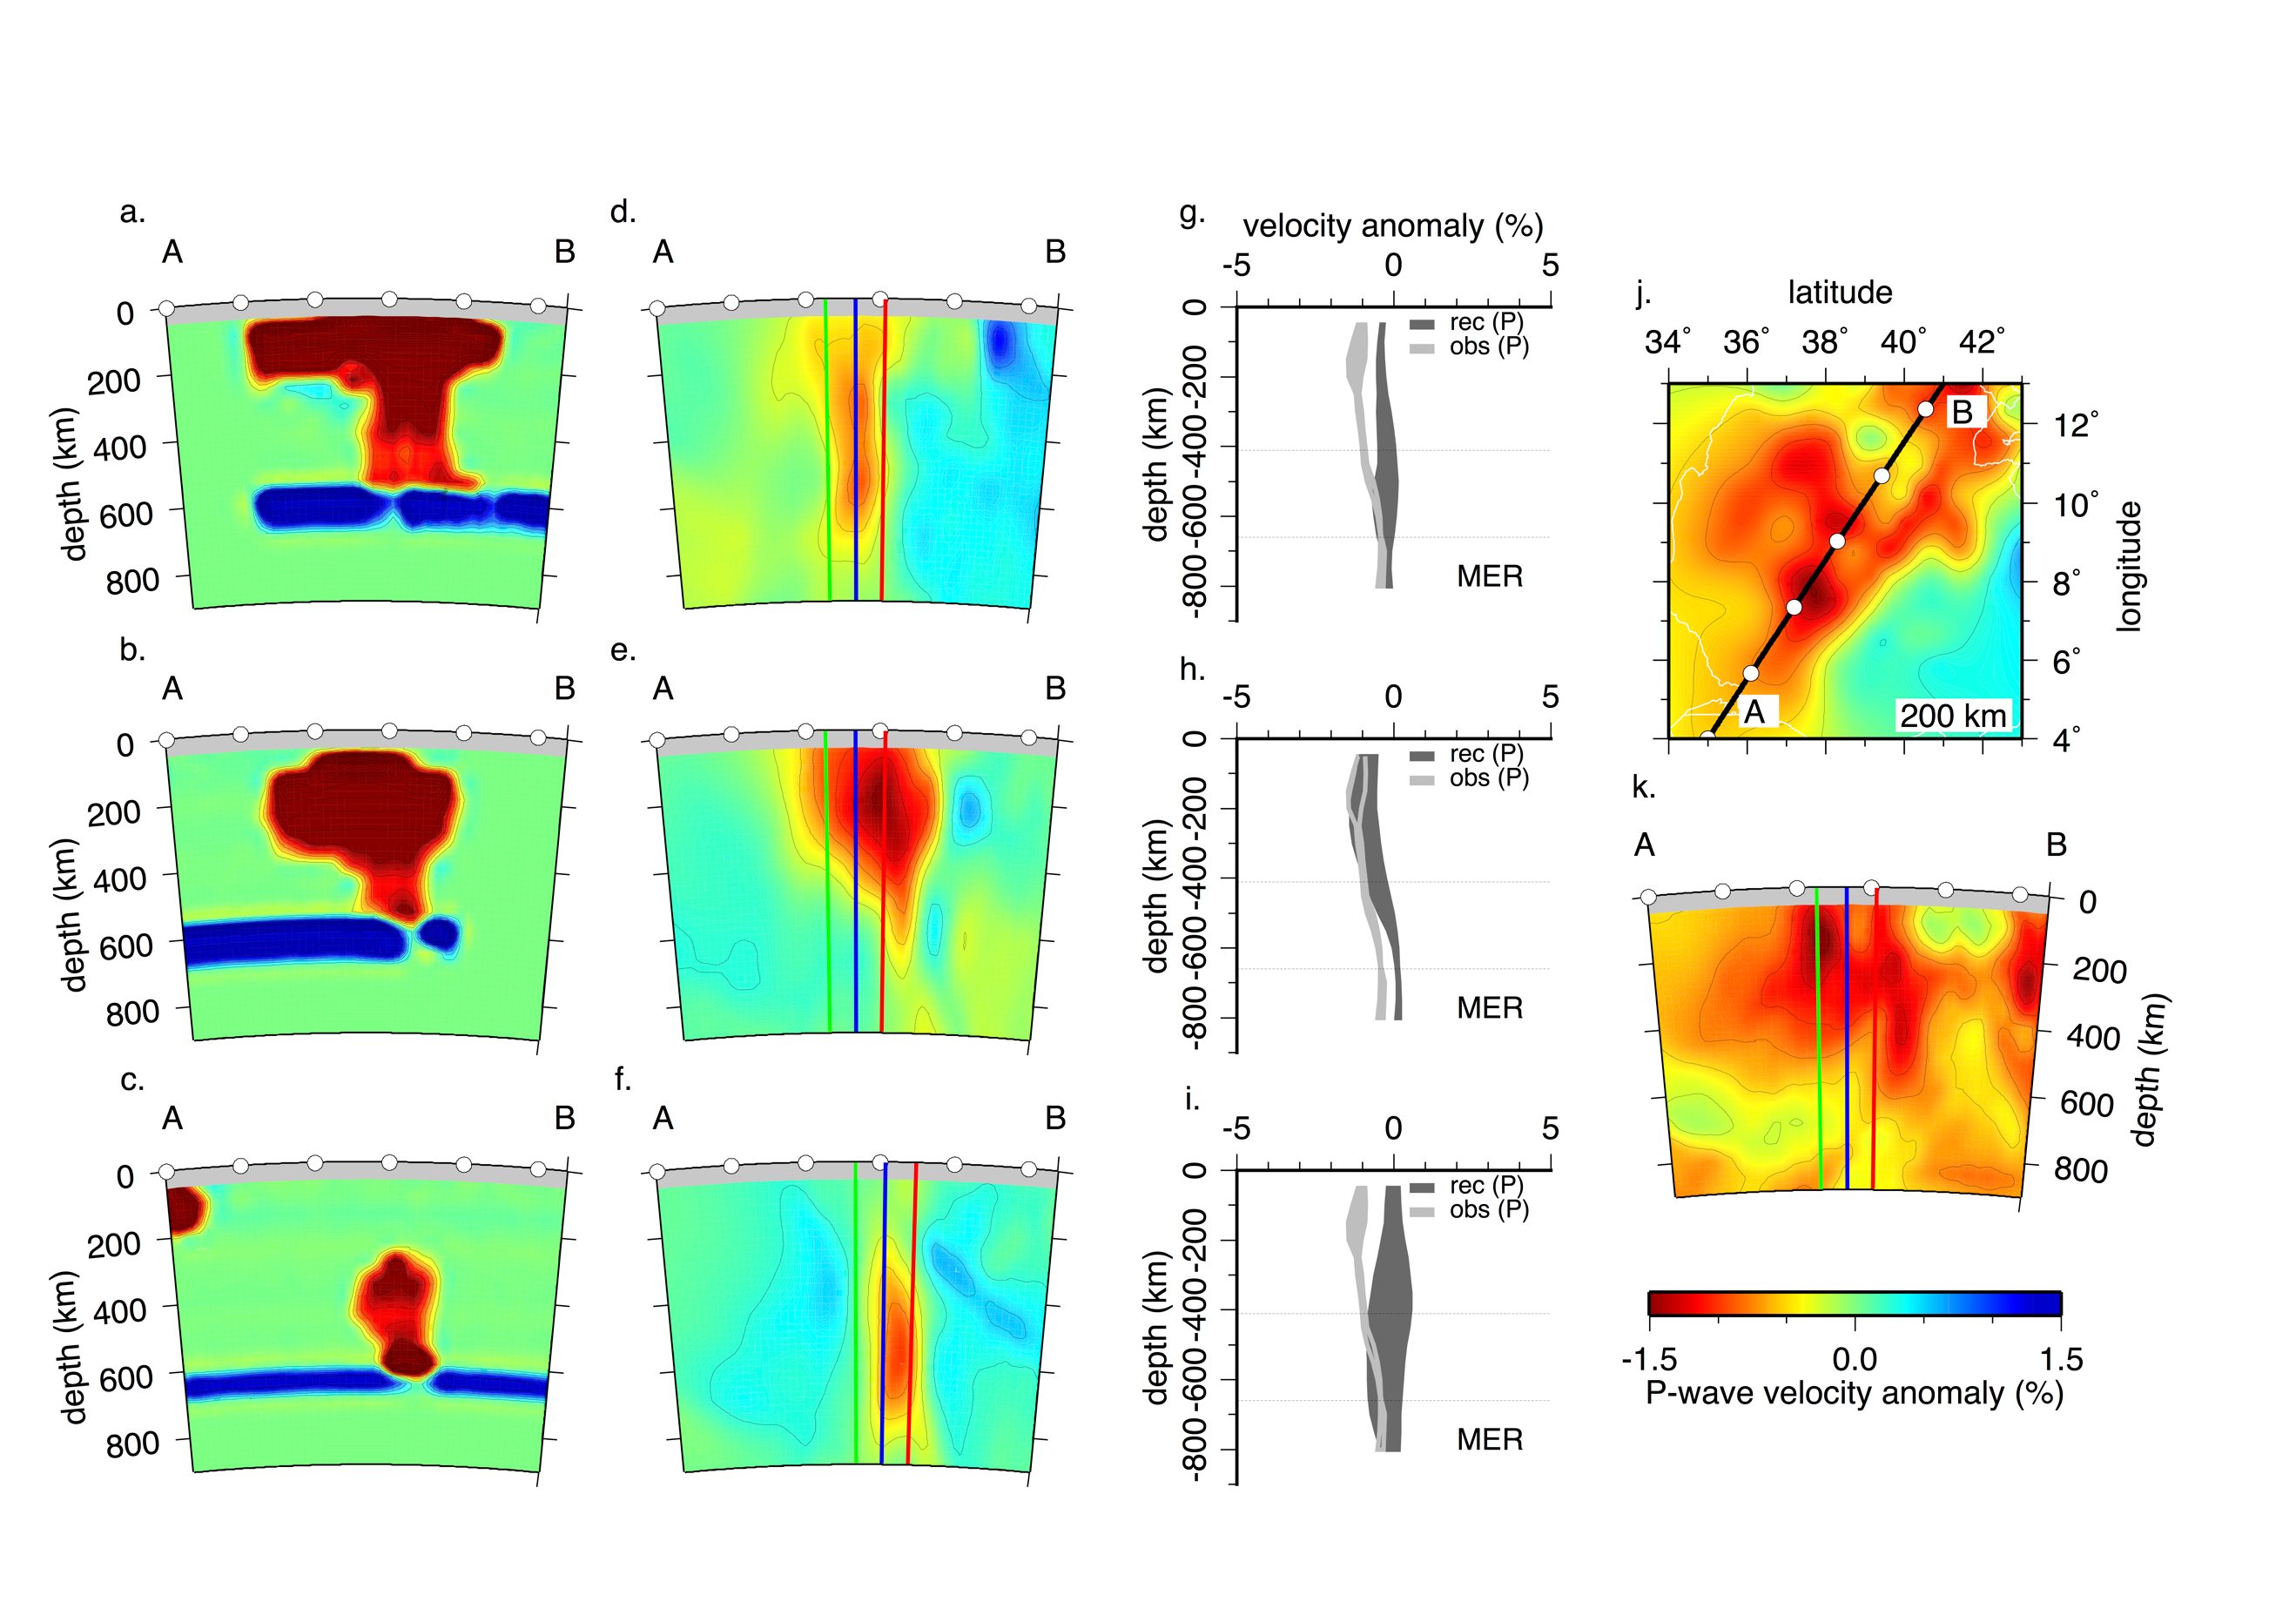
\includegraphics[width=16cm]{../figures-working/fig10.png}
\caption{Vertical cross-sections through the undamped P-wave model from model N9 with a $200\rm\,^{\circ}C$ hot layer, focused in the region below MER.  The orientation of the cross-sections (black line) is shown in the 200 km depth slices through the NEAR-P15 tomographic model  j.  (a, d) synthetic and resolved images of the LS phase of plume evolution; (b, e) synthetic and resolved images of the MS phase of plume evolution; (c-f) synthetic and resolved images of the ES phase of plume evolution. g-i) Input and retrieved P-wave velocity LS (g), MS (h) and ES (i) anomaly envelopes (\%) along the green, blue and red profiles drawn in the cross-sections. (j) 200 km depth slice through the undamped NEAR-P15 model k) Vertical cross-section of the undamped NEAR-P15 model. The spacing between the contours is 0.25\,\%. White points indicate the distance every $2^{\circ}$.}
\label{fg:9}
\end{figure*}

Using the model N9 that has a $200\rm\,^{\circ}C$ thermal anomaly as an example, we firstly positioned the ES, MS, and LS plumes in turn below the Afar and MER regions. In Figs.~\ref{fg:8} and \ref{fg:9} we show respectively the (undamped) P-wave models below Afar and MER. The same tests applying the moderate damping are illustrated in Supplementary Figs.~S2 and S3. The P-wave inversions of the dynamic models N8 and N10 are respectively shown in Supplementary Figs.~S4, S5 (undamped) and S6, S7 (damped) for Afar and Figs.~S8, S9 (undamped) and S10, S11 (damped) for MER region.

The recovered images for each plume stage are complex and therefore not straightforward to interpret without knowing the input model.
All the plume stems are resolved through the whole upper mantle, however without additional constraints on shallow structure, the retrieved images of the ES and LS plumes are very alike, particularly above 300\,km depth. This is due to the fact that the relative travel-time tomography does not have a good sensitivity to the shallow structure (0-200\,km). Thus, the head spreading at the base of the lithosphere in the LS case is almost completely lost in the inversion. Damping towards an alternatively constrained shallow structure, i.e. a 3D synthetic model down to a depth of 350\,km, helps to bring out the differences between the two structures (Figs.~S2, S3, S6, S7, S10 and S11). The MS plume appears more distinct from the ES and LS plumes in both undamped and damped inversions, as the upper-mantle head of the plume is broader and can be resolved laterally (Figs.~\ref{fg:8} and \ref{fg:9}). 

Overall, the modelled plumes in model N9 (temperature anomaly of $200\,^{\circ}$C) correlate well with the tomography-imaged features in terms of magnitude at transition-zone depths (see the profiles in Figs.~\ref{fg:8},\ref{fg:9}, S2 and S3). In comparison, the velocity amplitudes for a temperature anomally of $100\,^{\circ}$C (model N8) are weak compared to the observed structures (Figs. S4, S6, S8, S10), and the velocity amplitudes for a temperature anomally of 400°C (model N10) are almost double the observed seismic velocity anomaly (Figs. S5, S7, S9, S11). The instabilities originating from the high temperatures in model N10 are likely not realistic as the structure is too hot when compared to the seismic observations. It would appear that model N8 most closely matches the spatial and temporal distribution of the seismic features below the northern EAR, yet the destabilisation of a $200\,^{\circ}$C anomaly (model N9) best matches the velocity magnitudes.

\section{Discussion}

\subsection{Secondary plumes or destabilisation of ponded plume material}

We infer that a significant temperature excess from a thermal boundary layer is needed to match the amplitude of the upper-mantle low-velocity anomalies imaged in our observed tomography. Yet, it is difficult to reconcile the seismic signatures with a steady-state thermal boundary layer. The Rayleigh B{\'e}nard instabilities are either too diffuse (Newtonian models N1 to N4; Fig.~\ref{fg:3}a) or create anomalies that are too thin (non-Newtonian models N5 and N6; Fig.~\ref{fg:3}b), such that the thermal anomalies are seismically invisible or relatively weak \citep[e.g.][]{goes-etal-2004}. It is only for the Rayleigh Taylor models (N7 to N10) that thermal anomalies are sufficiently strong such that the seismic velocity anomaly is resolved in the synthetic tomography. This is a strong statement, as it implies that the plumelets are more than secondary thermal instabilities rising off a large whole mantle plume \citep[e.g.][]{kumagai-etal-2007,kumagai-etal-2008}. Rather the plumelets are of the same material as the large scale plume, which has stagnated at depth and then become sufficiently buoyant to rise further in the form of a Rayleigh Taylor-like destabilization.

A viscosity contrast in the mantle will act as a barrier to a thermal or thermo-chemical plume. This results in the heating of the boundary between the two layers, and the generation of secondary plumes \citep{kumagai-etal-2007}. This process is therefore similar to the Rayleigh B{\'e}nard numerical models in Fig. \ref{fg:2}, and Fig. \ref{fg:5}, which are either too diffuse or thin to be seismically imaged. Thermal-chemical plumes will stagnate if the compositional buoyancy is such that they become of equal density with the surrounding mantle. The chemical component of the plume will subsequently fall down back into the lower mantle \citep{kumagai-etal-2008}. It is possible that some of the chemical heterogeneity becomes entrained within the thermal upwelling, but again these plumes are not the equivalent of the Rayleigh Taylor numerical models that more closely match the seismic observations.

What we require is the arrival of some distinct buoyant material at between 1000 and 660\,km depth below East Africa, as for example imaged within the cluster analysis of five global S-wave tomographic models \citep{cottaar-2016}. This material subsequently destabilizes and rises to form the plumelets observed within the tomographic images. The arrival of deep plume material below the Afar is consistent with the Helium isotope record of this region, which is suggestive of the melting of a deep mantle source \citep{pik-etal-1999}. The volumetric quantity of this melting might signify a greater percentage of lower mantle than can be delivered by entrainement alone. Yet, the scenario of Rayleigh Taylor instabilities could occur if the large scale thermal-chemical plumes are also internally heated \citep{fourel-etal-2017}. In this case the large scale plume rises until it becomes neutrally buoyant. As it stagnates, internal heating will increase its temperature allowing for further destabilisation. The tomographic images of the upper mantle are most consistent with distinct, fat, thermal anomalies, which is consistent with models that include distinct density layers and internal heating \citep{fourel-etal-2017}. 

\subsection{Different or similar evolutionary stage plumes below Afar and MER?}

\begin{figure*}
\centering
\includegraphics[width=11cm]{../figures-working/fig11.png}
\caption{Resolution tests for the dynamic plume model N9 shifted and rotated so as to position a mid-stage plume below Afar and a later-stage plume west of the MER. a, b) Cross-sections of the synthetic (a) and resolved (b) P-wave MS plume located below Afar. The cross-section of the S-wave input plume is not shown as it is similar with higher amplitude. e, f) 200\,km depth slice (f) and cross-section (e) of the recovered plume. c, d) slice at 200 km depth (c) and cross-section (d) of the undamped P-wave tomographic model. g, h) slice at 200 km depth (g) and cross-section (h) of the undamped S-wave tomographic model. i, j) Cross-sections of the synthetic (a) and resolved (b) P-wave later-stage plume located below.}
\label{fg:10}
\end{figure*}

Comparing forward models with observed tomography to find a good matching between synthetic and observed features is not straightforward. Tomographic resolution is spatially variable and highly non-linear, making it difficult to assess \citep{rawlinson-etal-2010}. However, from our set of resolution tests for each plume stage of evolution, we clearly recognize that models with a strong tail, like ES and LS plumes, do not match our observations well in character or amplitude profiles with depth (Fig.~\ref{fg:8} and \ref{fg:9}).  Plumes in a middle phase of evolution (MS) with a broad head and a short tail best explain the evolutionary stage of both the upper-mantle structures below Afar and MER (Fig.~\ref{fg:10}). A MS plume below Afar matches the amplitude of both the P- and S-wave low-velocity anomalies within the transition zone and above (Fig.~\ref{fg:10} q, r). Moreover, the similarity between the retrieved and observed tomographic shape of the plume is striking, especially for the S-waves (Fig.~\ref{fg:10}). The plume below MER could be in a slightly more advanced stage with a pronounced head spread at the base of the lithosphere and a quite thin ($\sim 100$\,km diameter) tail. Yet given the simplicity of the Cartessian input model, we would still suggest that the structure below the MER represents a middle stage plumelet.

From our undamped synthetic models, the amplitude of the anomalies match quite well within the transition zone while in the uppermost mantle the observed tomographic images show much stronger anomalies compared to the synthetic models from synthetics (Fig.~\ref{fg:10} s, t). However, applying a moderate damping to the inversions in order to better retrieve the shallow velocity anomalies, we find a better match in amplitude between the models throughout the upper mantle (see Figure S13 s, t). In addition, in the damped case the shape of the anomaly is more consistent with the tomographic image of the MER plume, showing a largely widespread head in the topmost upper mantle, and a narrow stem within the transition zone. Overall, the resolution tests indicate that the two plumes below Afar and MER differ little in terms of geometry and similar stages of evolution are required to match the shapes and magnitudes.

The tomographic S-wave anomaly below Afar in NEAR-S16 is much stronger in velocity amplitude compared to that beneath MER. This prominent feature is not imaged in the recovered synthetic models. In addition, some localized strong low-velocity bodies appear in the upper mantle of our tomographic model below MER. To reconcile this seismic signature the strong low $V_{S}$ could be due to non-thermal heterogeneity such as melt retention in the upper mantle. As shown in the Supplementary Figure S14, we test the cases of a model with additional small-scale quantities of melt located directly below Afar and MER at different depth levels in the upper mantle at 75\,km and 185\,km depth \citep[c.f.][]{thompson-etal-2015}. Indeed, a signature of partial melt above the transition zone may be invoked as additional contribution to such velocity anomalies in order to match the S-wave anomalies, especially below Afar where the S-wave features are as strong as -5\,\%, almost double those below MER. The presence of melt at the lithospheric depths ($<50$-70\,km) would further enhance shallow anomalies adding to this contrast in anomaly strength. 

\section{Conclusions}

We find that the seismic structure seen in the upper mantle below Afar is similar in character, scale, and amplitude to what dynamic models predict for mantle plumelets originating from a $200\,^{\circ}$C excess temperature layer near the top of the lower mantle. This suggests that large scale mantle plumes rise upwards towards the upper mantle where they can stabilse. Subsequently due to the combination of chemical heterogeneity and internal heating, the structure will destabilise further into the upper mantle and express itself as plumelets with a spacing that is a function of the depth at which the structure stabilises and its width. Below East African Rift it would appear that the African Superplume stabilised at some point in the Earth's geological past at around 1000 to 660\,km, and subsequently it has destabilised and is currently rising beneath at least Afar and the Main Ethiopian Rift in the form of a Raleigh Taylor instability.

The synthetic tomography generated from the 3D models of Rayleigh Taylor instabilities highlight that plumes have complex signatures in tomographic images. This suggests that checkerboard tests and simple vertical cylindrical features used as model inputs are insufficient to test interpretations of tomographic images. In particular, if several small-scale plumes are active below a region, and they are in different stages of their evolution, as predicted in our dynamic models, there will be complexities in both geometry and amplitude of hte recovered synthetic tomography. This may explain the upper-mantle low-velocity anomalies that differ in shape from simple near-vertical cylindrical structures under a wide number of hotspot regions on scales of several 100\,km in the central Atlantic (Azores, Canaries, Cape Verde, Madeira and Great Meteor), an irregularly shaped anomaly of low P-wave velocities in the shallowest 200\,km, which slants northeast and downward to the top of the transition zone is imaged \citep{vinnik-etal-2012,yang-etal-2006}, beneath Central Europe where the low-speed anomalies show more than one branch in the upper mantle (Massif Central/Eifel; \citealp{granet-etal-1995,ritter-etal-2001} and Indian Ocean (Marion/Crozet) where several tilted upper-mantle upwellings are suggested to rise from transition-zone depths \citep{davaille-etal-2005,montelli-etal-2004a}. Given that other regions exhibit similarly complex upper mantle structure and/or spacing between volcanic centres, it would be worthwhile re-analysing some previously published tomographic images below hotspots in this light.



%Recent work (e.g., Civiero et al., 2015; Kumagai et al., 2007; Saki et al., 2015) has proposed that deep mantle plumes may lead to secondary small-scale upwellings in the upper mantle. The examples discussed in these studies reveal two spacing scales: (1) 1000-1500 km and (2) 50- few100 km. We propose that the latter scale may be the expression of upper-mantle plumelets, while the larger scale may correspond to branching that takes place in the lower mantle, as imaged by Rickers et al., (2013) and occurs in spherical numerical models (e.g., Davies et al., 2012). 
%We present here a set of tests based on dynamic models of upper-mantle plumelets with different mantle rheologies to evaluate how such upwellings might be resolved in regional teleseismic relative travel-time P- and S-wave tomography, using the configuration of sources and receivers from a recent study below the northern EAR (Civiero et al., 2016, 2015).
%The dynamic models reveal that the plume scale and spacing for reasonable upper-mantle rheologies is indeed in the range of the lower scales inferred from seismic images and spacing between volcanic centres at hotspots, although some variability in spacing occurs, again consistent with observations…..Add some more conclusions based on the results from the dynamic models.?
%Subsequently, we perform resolution tests on the set of models with different spacing and amplitude to compare with those inferred from the tomography below Afar by Civiero et al., (2016, 2015). We convert the plumes’ thermal structure into seismic structure taking into account the effect of temperature, pressure, phase and anelasticity. Then we carry on synthetic tomography using the distribution of stations and sources and regularisation that was applied in our P- and S-wave tomography below the northern EAR.
%We find that: 
%(1) The tomographic tests of the synthetic plumes share many characteristics with the actual structures retrieved from P and S data in Civiero et al., (2015, 2016) including a similar scale, similar degree of variability in shape of the anomalies, similar amplitude and similar reduced correlation towards the base of the transition zone. The destabilisation of a 100C, 100 km thick thermal anomaly at ~700 to 800 km depth with a non-Newtonian rheology, most closely matches the spatial and temporal distribution of seismic anomalies below the northern EAR. However, the destabilisation of a 200C anomaly best matches the magnitudes of the instabilities in the upper mantle.
%(2) The comparison between the tomographic models NEAR-P15 and NEAR-S16 and the resolution tests of the synthetic plumes indicate the thermal boundary layer cannot be placed neither above the transition zone and deep in the lower mantle. The analysis of the vertical correlation functions of the plume models are characterised by a strong decrease in correlation in the thermal boundary layers at the top and base of the model. Together these findings strengthen our interpretation that the upper-mantle structure below the rift system is the result of small-scale upwellings rooted in a local thermal boundary layer in the topmost lower mantle, just below the ‘660’.
%(3) Plumes at different stages, from starting plumes with a small head (ES) to a late stage plume where the tail has thinned and head spread below the lithosphere (LS), are not easy to distinguish with teleseismic travel-time tomography, which has little sensitivity to the heads at shallow depth. Constraints on shallow structure (e.g., from surface waves) are needed to distinguish the stage of evolution of a plume.
%(4) From the analysis of both undamped and damped P- and S-wave models the plumes below Afar and MER seem to be in a similar middle stage of evolution, showing a significant head and a quite thick and short tail. Nonetheless, slightly stronger low-velocity anomalies are imaged below Afar than MER, indicating that the upwelling below MER may be likely in a slightly later stage, i.e., with thinner stem and spread-out head at the base of the lithosphere.
%In conclusion, these synthetic tests highlight that plumes may have more complex signatures in tomographic images than the simple vertical cylindrical features that are commonly searched for, even if they are purely thermal. In particular, if several small-scale plumes are active below a region and are in different stages of their evolution, this may lead to complexities in both geometry and amplitude.

\section*{Acknowledgments}
CC was supported by a Janet Watson Fellowship from the Department of Earth Science and Engineering at Imperial College, JA is funded by ANR Accueil de Chercheurs de Haut Niveau grant InterRift. GMT \citep{wessel-1995} software was used to plot Figs.~\ref{fg:1}, and \ref{fg:7} to \ref{fg:10}.

\bibliography{ref}

\end{document}